\section{Let's the fun begin!}
\newthought{We are left to define derivatives} of functions between manifolds.
And, since we saw that euclidean spaces are manifolds, we better find a definition that coincides with the one you saw in your analysis courses.

\begin{marginfigure}[7em]
  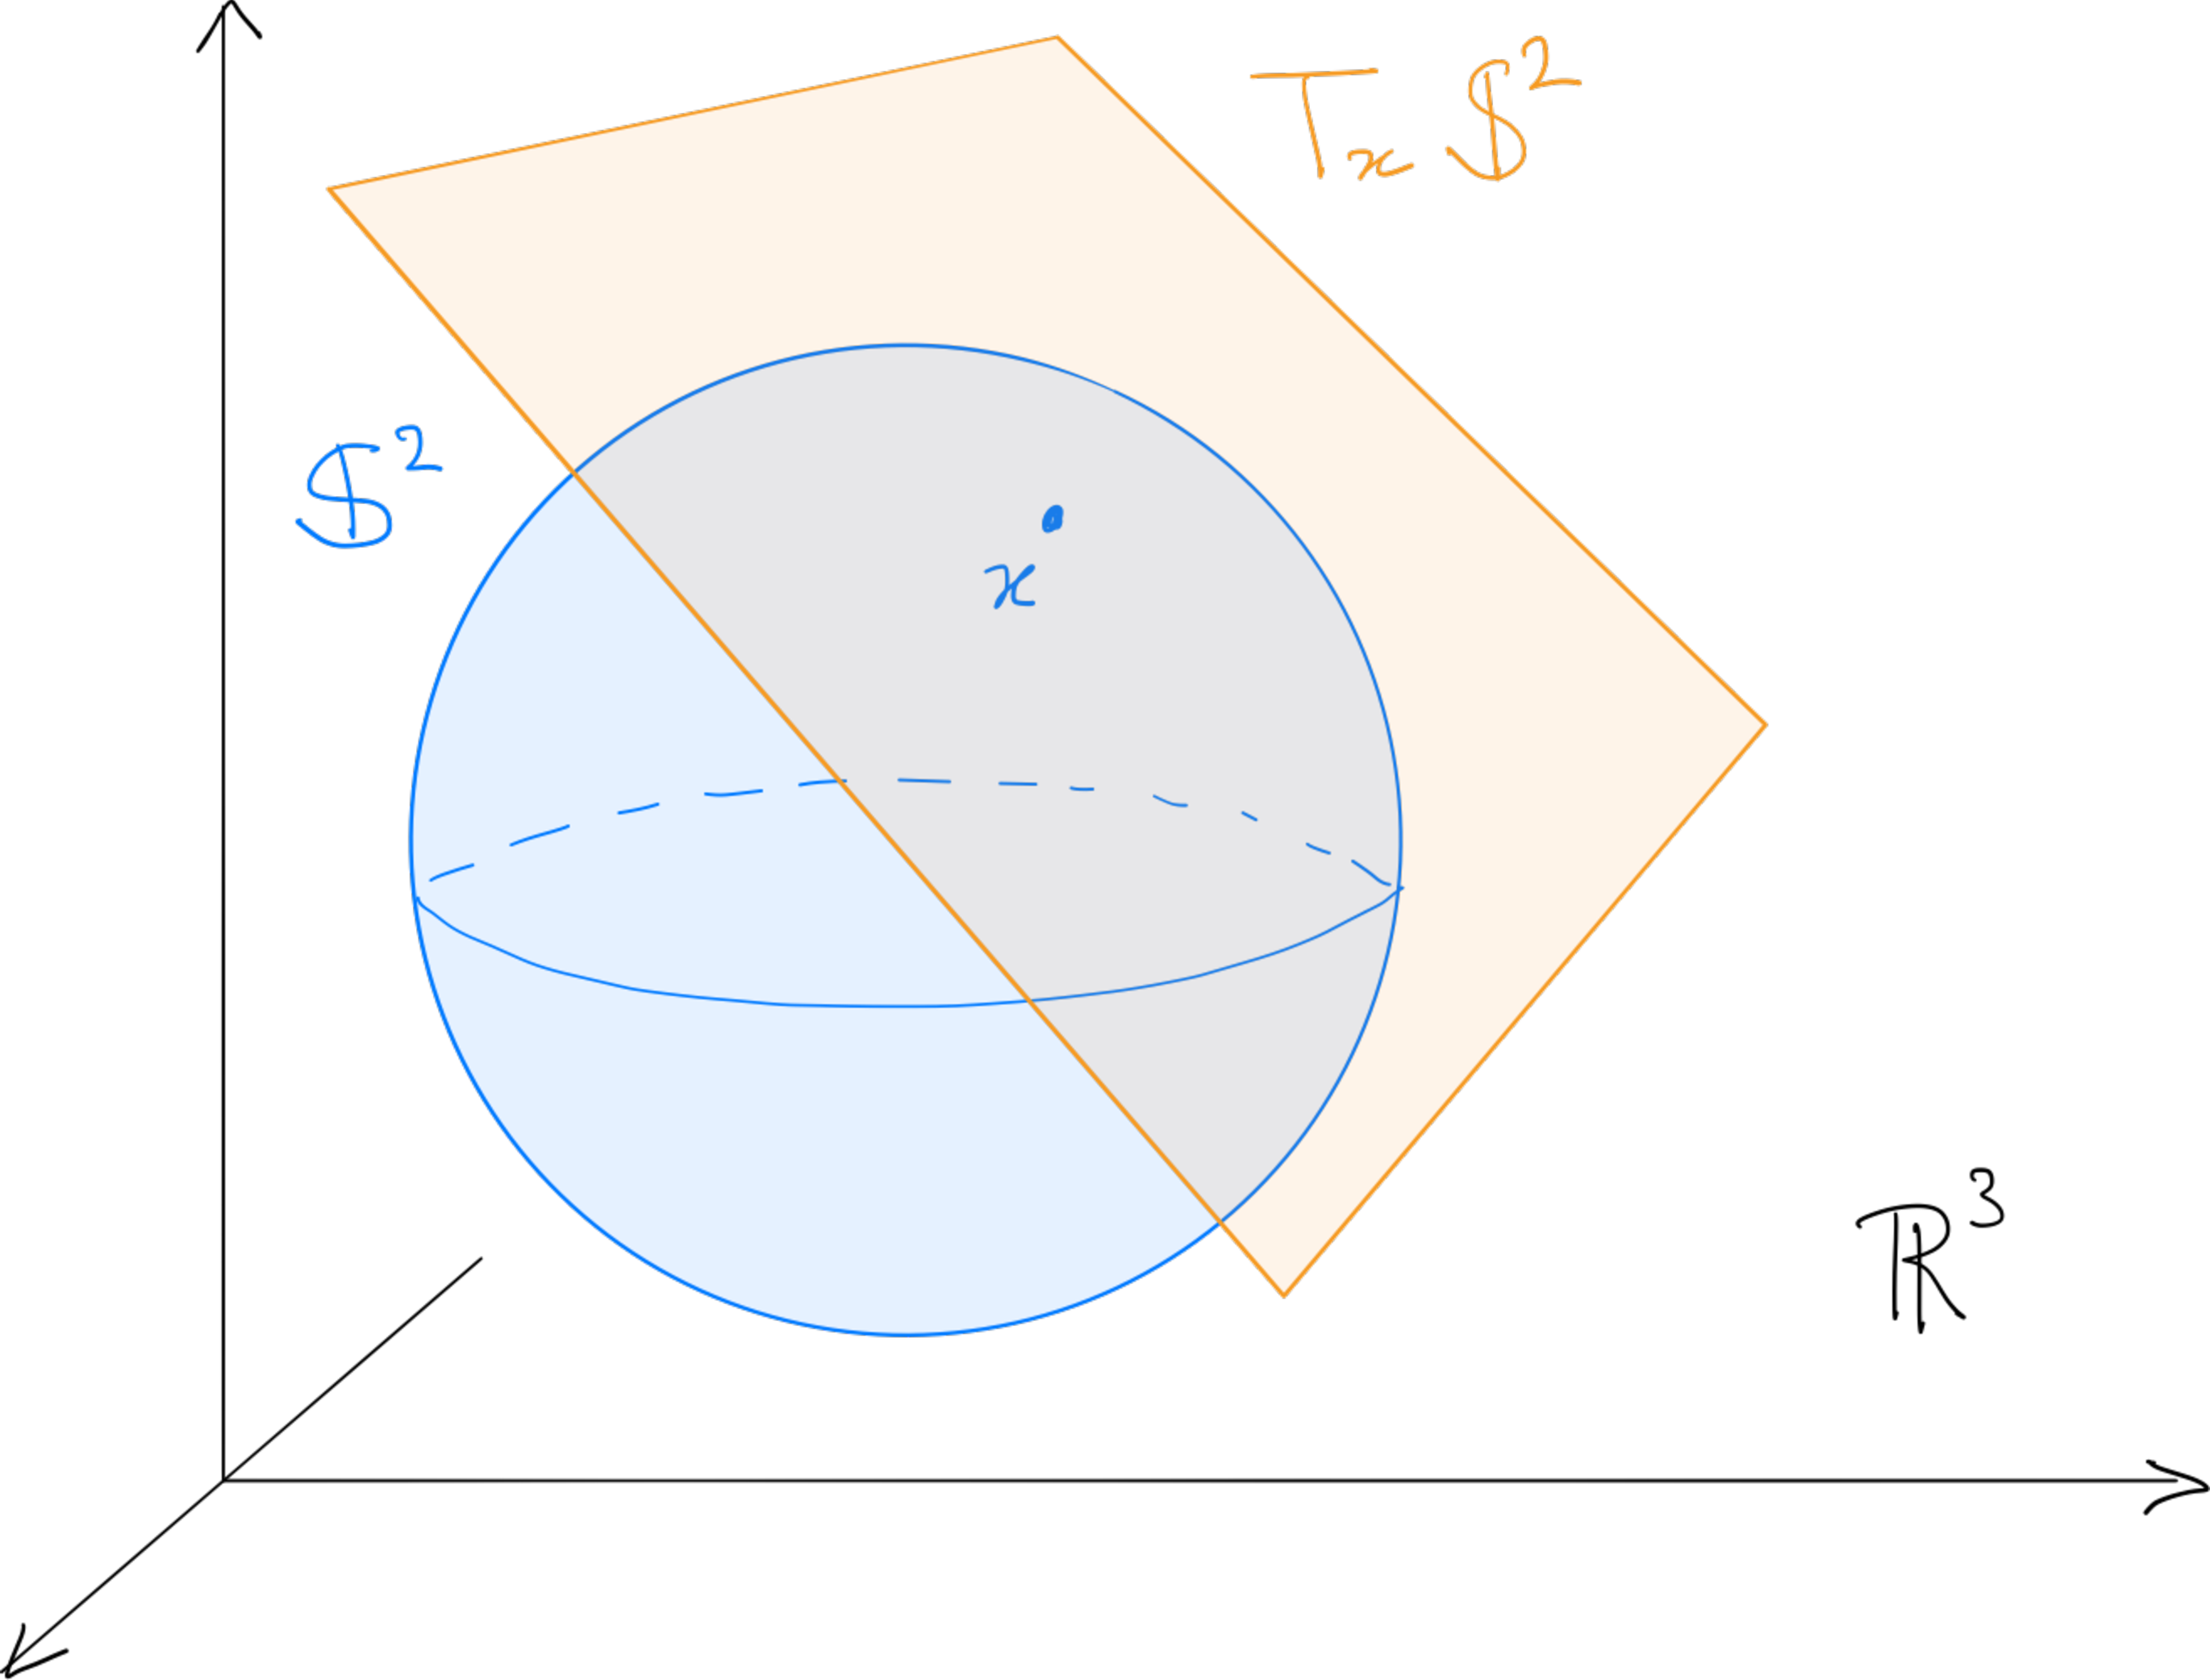
\includegraphics{2_1-embedded-sphere-tangent.pdf}
  \label{fig:tan-embedded-sphere}
  \caption{Tangent space to a point of a sphere $\bS^2$ embedded into the ambient space $\R^3$.}
\end{marginfigure}
In this chapter we will see how to associate to an $n$-dimensional smooth manifold $M$ an $n$-dimensional vector space, denoted by $T_x M$, to each point $x\in M$.
Such vector space is called \emph{tangent space to $M$ at $x$} and, for a manifold embedded into a euclidean ambient space, it will coincide with the intuitive understanding of a tangent hyperplane to the point on the manifold, see also Figure~\ref{fig:tan-embedded-sphere}.
As we will see, there are various different definition of tangent space but, in the end, they all turn out to be equivalent.

Due to the amount of freedom and the many equivalent definitions, there is no unique way of introducing tangent spaces.
Just to give you an idea, all the following approaches lead to equivalent definitions (see also \cite{book:lee}):
\begin{enumerate}
  \item equivalence classes of curves through a point;
  \item transformation laws of the components of vectors with respect to different charts;
  \item generalization of linear approximation into the idea of an abstract derivation;
  \item derivations in the category of germs of functions;
\end{enumerate}

It is also possible to ``flip'' the whole construction around, constructing differentials and cotangent spaces and using them to introduce the tangent spaces.
This is the approach taken by \cite{lectures:hitchin} and it is at least worth of a look if you want to see a different perspective.

To avoid diverging from the book too much, we will stick to derivations on the space of germs, which emphasizes the locality of derivations to an extreme.
The equivalence between our approach and the one based on speeds of curves and on derivations will be left as homeworks.

\section{Directional derivatives in euclidean spaces}\label{sec:dd}

Suppose that $f: U\subset\R^n\to\R^k$ is a smooth map defined on an open subset $U\subset \R^n$.
In multivariable calculus you have seen that if $x\in U$ and $v\in\R^n$, then the vector $Df(x) v$ can be interpreted as the directional derivative\footnote{Sometimes this is denoted $D_v f(x)$ instead.} of $f$:
\begin{equation}
  Df(x) v = \lim_{t\to0}\frac{f(x+tv) - f(x)}{t}.
\end{equation}
Then, the partial derivative is obtained as the particular case
\begin{equation}
  D_jf(x) := Df(x) e_j = \lim_{t\to0} \frac{f(x+te_j) - f(x)}{t}.
\end{equation}
Of course, we can also look at the derivative by using the standard euclidean coordinates $r^1, \ldots, r^n$, in that case we would be deriving $r^i \circ f : \R^n \to \R$.

\newthought{Let's take it slow}, and compare all these various derivatives next to each other.
For $f:U\subset\R^n\to\R^k$ and $x\in U$, we have
\begin{marginfigure}[3.5cm]
  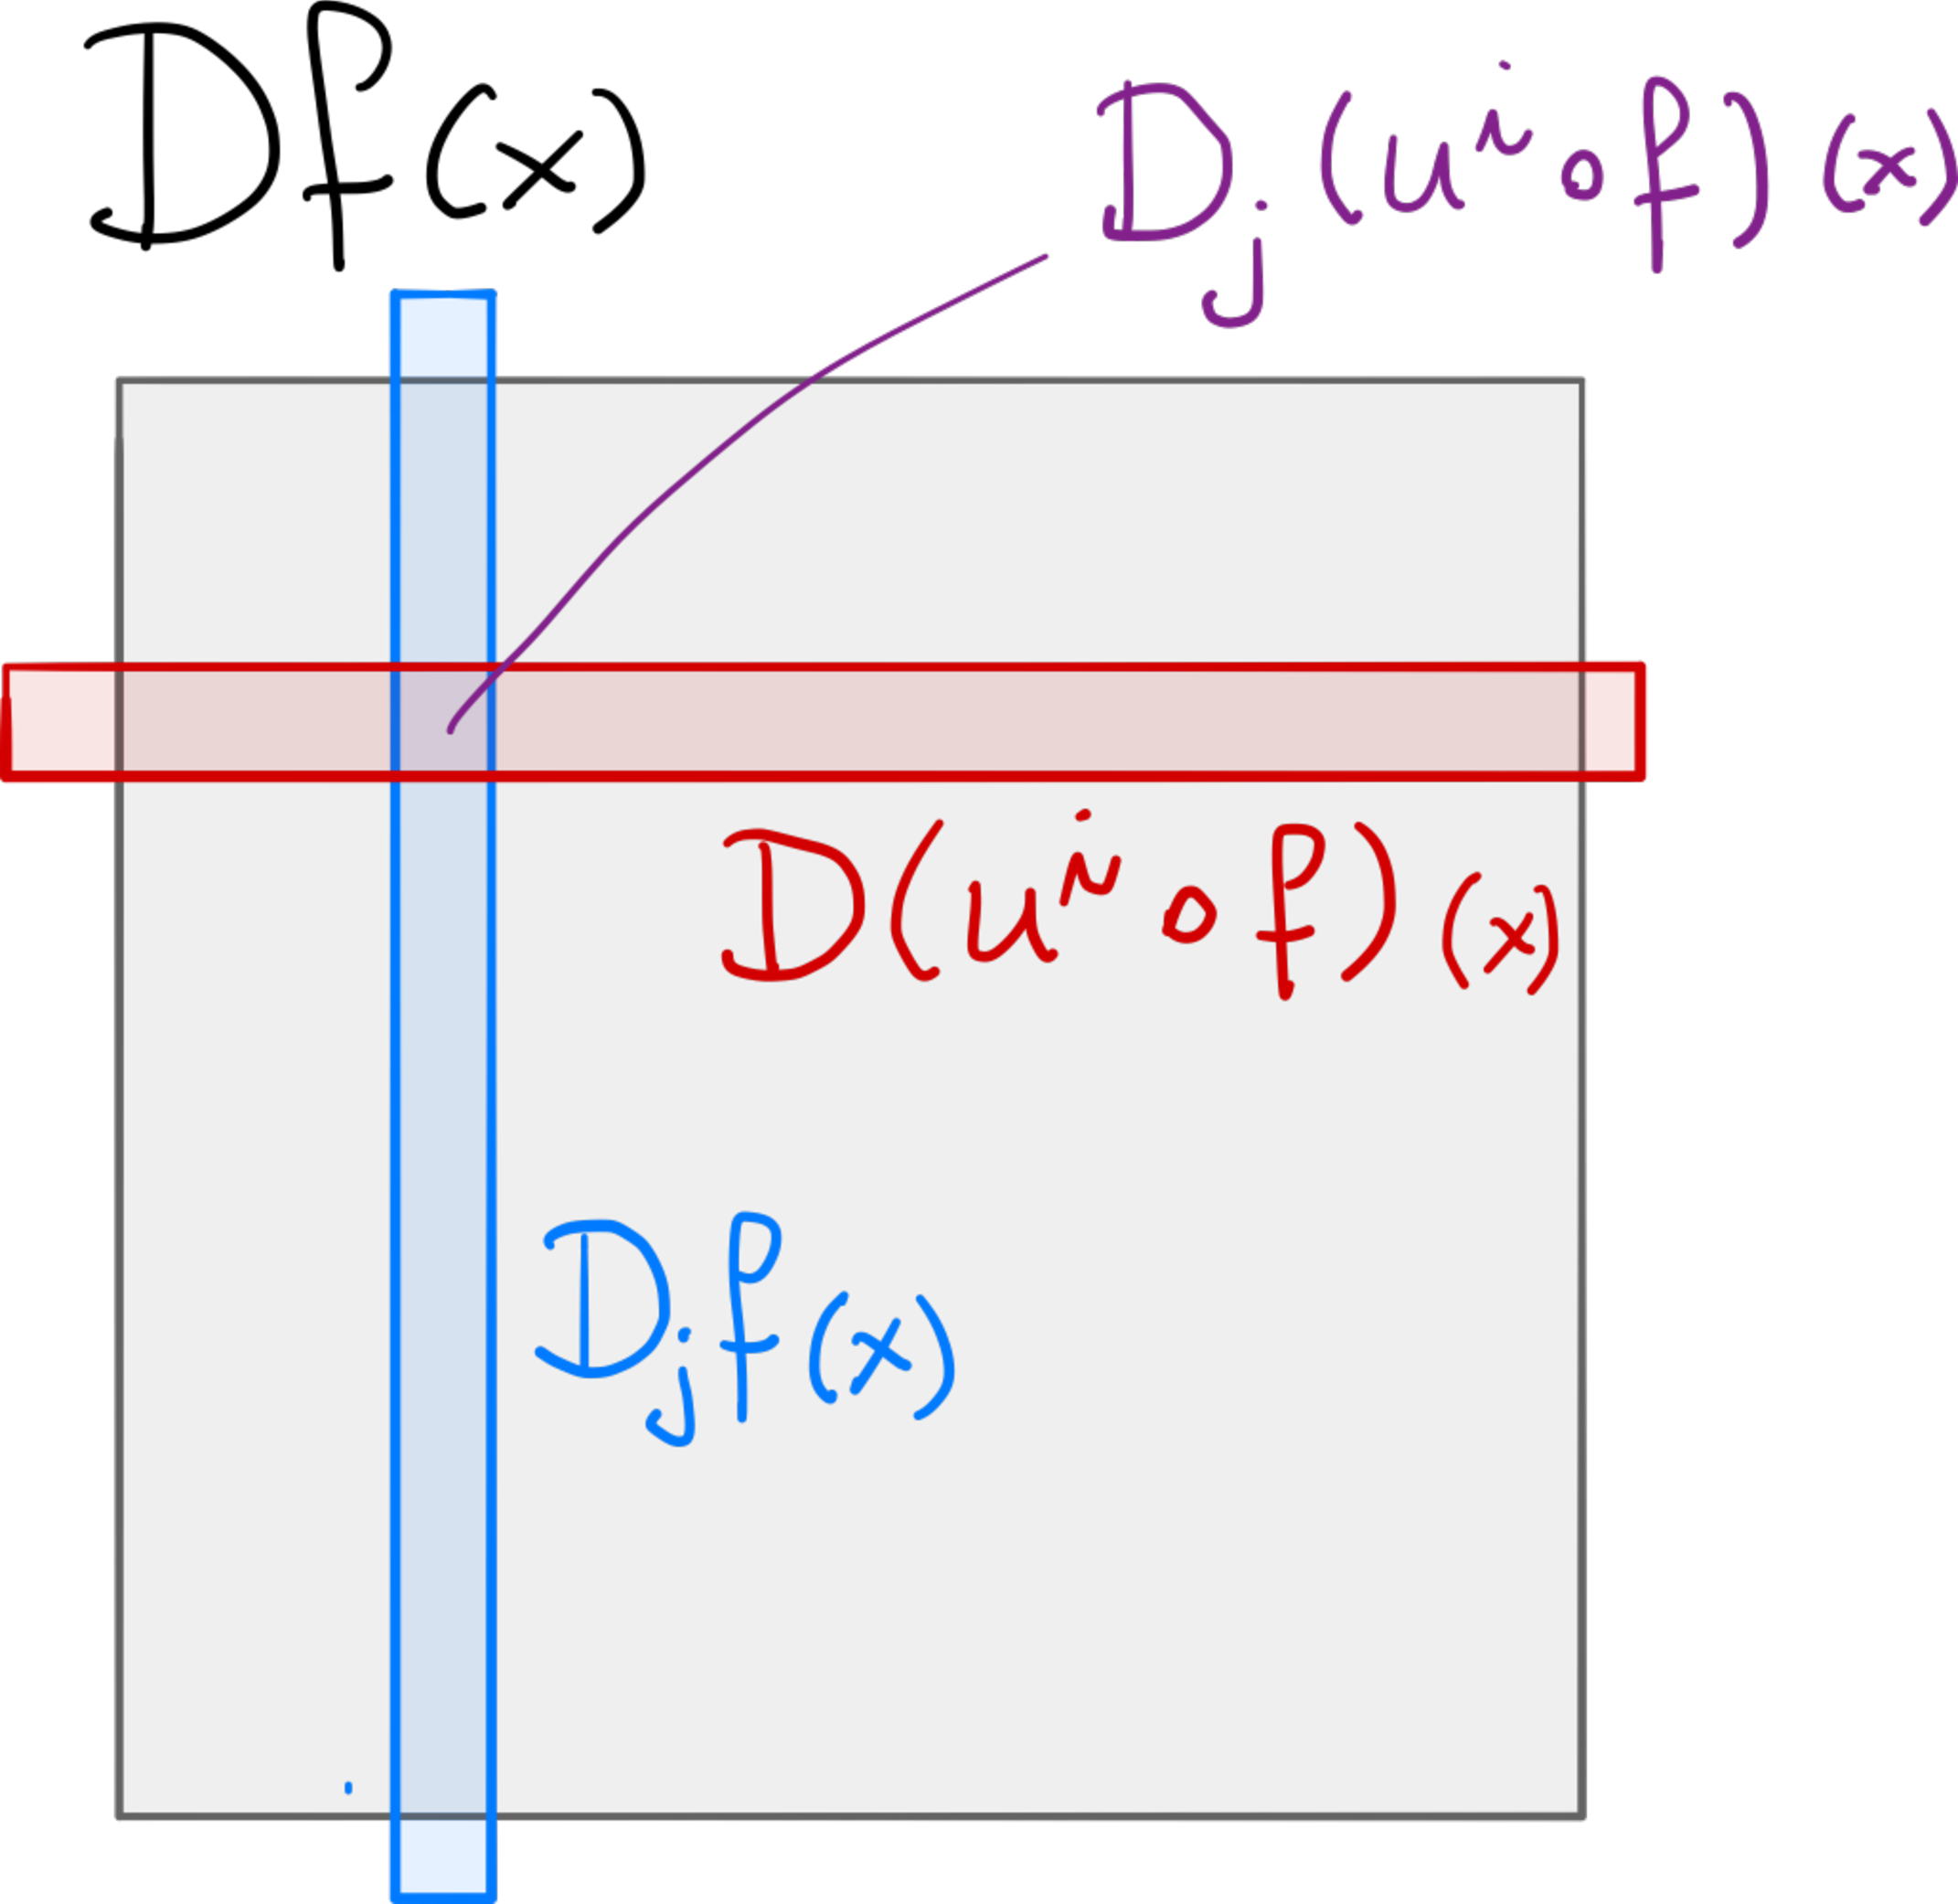
\includegraphics{2_3-ederivs.pdf}
\end{marginfigure}
\begin{itemize}
  \item $Df(x)$, the Jacobian matrix, which is a $k\times n$ matrix;
  \item $D_j f(x)$, the $j$th column of the matrix $Df(x)$, which is an element of $\R^k$;
  \item $D(r^i\circ f)(x)$, a linear function from $\R^n to \R$, which one can think as the $i$th row of the matrix $Df(x)$;
  \item $D_j(r^i\circ f)(x) = \frac{\partial f^i}{\partial x^j}(x)$, a number in $\R$, which corresponds to the element $(i,j)$ of the matrix $Df(x)$.
\end{itemize}

This notation using $D$ instead of spelling out the partial derivatives, comes with an important advantage.
Let's use it to rewrite the chain rule form Proposition~\ref{thm:chainrule}(\ref{thm:chainrule2}):
\begin{equation}
  D_j(u^i\circ g \circ f) (x) = \sum_{r=1}^k D_r(u^i\circ g)(f(x))\; D_j(u^r \circ f)(x),
\end{equation}
\marginnote[-4em]{Using Einstein notation, since $r$ is the only index that appears both in lower and upper position, $D_j(u^i\circ g \circ f) (x) = D_r(u^i\circ g)(f(x))\; D_j(u^r \circ f)(x)$.}
where $1\leq i\leq m, 1\leq j \leq n$.
As you cen see, we did not need to spell out explicitly the coordinate systems on $\R^n$ or $\R^k$.

\section{Germs and derivations}

\newthought{To reach our goal of defining derivations on manifolds}, a direct extension of partial derivatives is not enough: we will need to introduce some more levels of abstraction.

\begin{definition}
  Let $M$ be a smooth manifold.
  For some point $p\in M$, let $U,V\subset M$ be two neighborhoods of $p$.
  We say that two functions $f\in C^\infty(U)$ and $g\in C^\infty(V)$ have the same \emph{germ} at $p$ if there exists a neighborhood $W\subset U\cap V$ of $p$ such that $f|_W \equiv g|_W$.
\end{definition}

Germs define an equivalence relation on the set of smooth functions defined on a neighborhood of a point $p$: $(U, f) \sim_p (V, g)$ if they have the same germ at $p$. Then, a germ $[f]_p$, where $(U, f)$ is one representative for $[f]_p$, is an equivalence class in the quotient space 
\begin{equation}
  C_p^\infty(M) := C^\infty(M)/\sim_p.
\end{equation} 

\begin{exercise}
  Show that $\sim_p$ defined above is an equivalence relation in $C^\infty(M)$.
\end{exercise}

For $c\in\R$ and $[f]_p, [g]_p$ germs with representatives $(U, f), (V, g)$, we have
\begin{itemize}
  \item $[f]_p + [g]_p$ is the germ with representative $(U\cap V, f+g)$;
  \item $[f]_p [g]_p$ is the germ with representative $(U\cap V, f g)$;
  \item $c[f]_p$ is the germ with representative $(U, cf)$.
\end{itemize}
Therefore, $C_p^\infty(M)$ is also an algebra over $\R$.

Germs are the apotheosis of locality: a germ at $p$ has a well defined value at $p$ and nowhere else.
This results in a map,
\begin{equation}
  \eval_p: C_p^\infty(M) \to \R, \quad
  \eval_p([f]_p) := f(p),
\end{equation}
where $(V,f)$ is any representative of $[f]_p$.

We can now go back to our discussion of euclidean derivations to motivate our definition of tangent vectors.

\begin{example}\label{ex:euclideanD}
  Let $U\subset\R^n$ open\footnote{In what follows, we will think at $U$ both as an open subset of $\R^n$ and a smooth manifold depending on what is most convenient for us.} and $f\in C^\infty(U)$.
  For $x\in U$ and $v\in\R^n$ we have seen that $Df(x)$ can be interpreted as a matrix that consumes the vector $v$ to produce a number $D(f)v$.
  In such interpretation $f$ is fixed and only $x$ and $v$ vary, however there is no reason for this restriction.

  Indeed, an alternative interpretation lets also $f$ vary and consider the action of differentiation as a map
  \begin{equation}
    U \times \R^n \times C^\infty(U) \to \R,\quad
    (x,v,f) \mapsto Df(x) v.
  \end{equation}
  And since we are flipping around all the ideas, let us consider $x$ and $v$ fixed and instead only let $f$ vary:
  \begin{equation}\label{eq:mapxvtoD}
    (x,v):C^\infty(U) \to\R, \quad (x,v)(f) := Df(x)v.
  \end{equation}.
  By the definition \eqref{eq:diff} of the euclidean differential, we know that it is a local property: the value $Df(x)$ only depends on the germ of $f$ at $x$.
  Thus we can rephrase \eqref{eq:mapxvtoD} by saying that $v$ defines a \emph{linear} map
  \begin{equation}
    v : C_p^\infty(U) \to \R, \quad
    v([f]_p) := Df(x) v.
  \end{equation}
  In fact, this is not just a linear map, it also satisfies a \emph{derivation} property, in the sense that
  \begin{equation}
    v([f]_p [g]_p) =
      \eval_p([f]_p)v([g]_p)
      + \eval_p([g]_p)v([f]_p).
  \end{equation}
  Which, rewritten in a more familiar form, is just a way to rewrite the \emph{Leibniz rule}:
  \begin{equation}
    D(fg)(x) v = f(x)Dg(x)v + g(x) Df(x)v.
  \end{equation}

  Note that we have now two different interpretations for $v$: it is both a vector in $\R^n$ and a linear map $C_p^\infty(U) \to \R$ satisfying the derivation property.
\end{example}

Motivated by Example~\ref{ex:euclideanD}, we will define a tangent vector as a derivation on the space of germs.

\begin{definition}
  Let $M$ a smooth manifold of dimension $n$ and let $p\in M$.
  A \emph{tangent vector at $p$} is a linear map
  \begin{equation}\label{def:tangentvector}
    v: C_p^\infty(M)\to\R
  \end{equation}
  which is also a derivation, i.e.
  \begin{equation}
    v([f]_p [g]_p) =
      \eval_p([f]_p)v([g]_p)
      + \eval_p([g]_p)v([f]_p).
  \end{equation}

  Since a tangent vector is a linear map from the vector space $C_p^\infty(M)$ to $\R$, the set of all tangent vectors at a point $p$ is itself a vector space\footnote{Exercise: why is this true?} which we denote by $T_p M$.
\end{definition}

Let's check that these vectors, at least satisfy the most elementary properties of derivations: one would expect the derivative of constant functions to be zero, is that the case?

\begin{lemma}\label{lem:f'0is0forconst}
  Let $M$ be a smooth manifold, let $U\subset M$ be an open set containing $p$ and let $v\in T_p M$.
  Denote by $[c]_p$ the germ of a constant function $(U, p \mapsto c)$.
  Then $v([c]_p) = 0$.
\end{lemma}
\begin{proof}
  Since $[c]_p = c [1]_p$, by linearity we have $v([c]_p) = c v([1]_p)$.
  Thus, it will be enough to show that $v([1]_p) = 0$.
  Since $v$ is a derivation, using the algebra properties of the space of germs we get
  \marginnote{Keep this simple trick in mind, it will be useful in the future.}
  \begin{equation}
    v([1]_p) = v([1]_p [1]_p) = 2 \eval_p([1]_p)v([1]_p) = 2 v([1]_p).
  \end{equation}
  Thus, $v([1]_p) = 0$, concluding the proof.
\end{proof}

As you can see, working with equivalent classes is doable but unnecessarily cumbersome. As we did with atlases, we would like to get it over with.

\begin{definition}
  Let $M$ be a smooth manifold and $p\in M$.
  Let $W\subseteq M$ be any neighborhoods of $p$.
  A \emph{derivation of $C^\infty(W)$ at $x$} is a linear map $w:C^\infty(W)\to\R$ which satisfies Leibniz rule
  \begin{equation}
    w(fg) = f(p)w(g) + g(p)w(f).
  \end{equation}
\end{definition}

If $v\in T_p M$, then we already saw that $v$ naturally defines a derivation $w$ of $C^\infty(W)$ for any open neighborhood $W$ of $p$.
In this case
\begin{equation}\label{eq:derivfromtg}
  w(f) := v([f]_p).
\end{equation}
Showing that the opposite is also true will require a bit of work.

\begin{proposition}
  Let $M$ be a smooth manifold, $p\in M$ and $W$ any neighborhood of $x$.
  Then there is a linear isomorphism between $T_p M$ and the space of derivations of $C^\infty(W)$ at $p$.
\end{proposition}
\begin{proof}
  To prove the theorem we need to invert \eqref{eq:derivfromtg} and define a tangent vector in terms of of a derivation of $C^infty(W)$ at $p$.
  We will proceed in three steps

  \newthought{Step I}. Let $w:C^\infty(W) \to\R$ be a derivation at $p$ and suppose that $f\in C^\infty(W)$ is identically zero on a neighborhood $W_0\subset W$ op $p$. We are going to show that $w(f)=0$.

  By Proposition~\ref{prop:cutoff}, we can find a function $\rho:M\to\R$ such that $\rho(p)=1$ and $\supp(\rho) \subset W_0$. Consider now $g = \rho f : W \to \R$. Then $g$ is identically zero in the whole $W$, and thus\footnote{Follows by linearity, exactly as in Lemma~\ref{lem:f'0is0forconst}} $w(g) = 0$. Using Leibniz rule, the fact that $\rho(p)=1$ and $f(p) = 0$, we get
  \begin{equation}
    0 = w(g) = w(\rho f) = \rho(p) w(f) + f(p)w(\rho) = w(f).
  \end{equation}

  \newthought{Step II}.
  Let $[f]_p\in C_p^\infty(M)$.
  We want to show that it is always possible to find a representative for $[f]_p$ with domain $W$, that is, there exists $g\in C^\infty(W)\to\R$ such that $[g]_p = [f]_p$.
  Let $(V, f)$ be any representative of $[f]_p$.
  Since germs are local, if necessary, we can shrink $V$ so that $V\subset W$.
  Here comes the tricky bit: we need to extend $f$ to a function $g$ defined on $W$ which coincides with $f$ in some neighborhood of $p$!
  To this end, choose\footnote{We can do this because topological manifolds are locally compact Hausdorff spaces, which implies that every point has a neighborhood with compact closure.} a smaller neighborhood $U$ of $p$ such that $\overline{U}\subset V\subset W$.
  Again, Proposition~\ref{prop:cutoff} comes to the rescue. Apply it with $K=\overline{U}$ and ``$U$'' equal to $V$, and consider
  \begin{equation}
    g:W\to\R, \quad
    g(q) := \begin{cases}
      \rho(q)f(q), & q\in V,\\
      0, & q \in W\setminus V.
    \end{cases}
  \end{equation}
  Since $g|_U = f$, we have $[g]_p = [f]_p$, proving the claim.

  \newthought{Step III}. We can now complete the proof.
  Let $w:X^\infty(W) \to\R$ be a derivation at $p$.
  A tangent vector is a linear map $v:C_p^\infty(M)\to\R$, see \eqref{def:tangentvector}, and a derivation.
  We would like to define one in terms of $w$.
  Given any $[f]_p\in C_p^\infty(W)$, the previous step guarantees that there exists a representative $(W,f)$ for it, so we can define
  \begin{equation}
    v([f]_p) := w(f), \quad\mbox{where $(W,f)$ is any representative of $[f]_p$}.
  \end{equation}
  Such $v$ is a derivation by construction, so if it is well-defined, we are done.
  To this end, assume that there exists a different representative $(W, g)$ for $[f]_p$.
  Then, by definition, there exists a neighborhood $V\subset W$ of $p$ such that $f|_p = g|_p$.
  By linearity, $w(f) - w(g) = w(f-g)$ and by the first step in the proof, $w(f-g) = 0$.
  
  The assignment $w\mapsto v$ inverts \eqref{eq:derivfromtg}, completing the proof.
\end{proof}

This seemingly innocent proposition, has some very important consequences.

First of all, from now on we are free to interpret tangent vectors in $T_p M$ as derivations of $C^\infty(W)$ at $p$ for \emph{any}\footnote{In particular, it is often convenient to have $W$ coincide with the domain of a chart or with the whole manifold $M$.} open $W$ containing $p$.
This enables us to give our first example of tangent vector.

\begin{example}\label{ex:partialderivative}
  Let $M$ be a smooth manifold of dimension $n$ and $\phi: U \to V$ a chart on $M$.
  As already mentioned, we write $x^i = r^i \circ \phi$ for the local coordinates\footnote{See Notation~\ref{ntn:coords}.} of $\phi$.
  For any $p\in U$, we can define a derivation of $C^\infty(U)$ at $p$ as
  \begin{equation}
    \frac{\partial}{\partial x^i}\Big|_p : C^\infty(U) \to \R, \quad
    \frac{\partial}{\partial x^i}\Big|_p (f) := D_i(f\circ\phi^{-1})(\phi(p)).
  \end{equation}
  We will soon see that $\left\{\frac{\partial}{\partial x^i}\Big|_p \mid 1\leq i\leq n\right\}$ forms a basis for $T_p M$.
\end{example}

Secondly, it provides us some very useful corollaries.

\begin{corollary}\label{cor:tgsubspace}
  Let $M$ be a smooth manifold and let $W\subset M$ be a non-empty open set considered as a smooth manifold.
  Then, for any $p\in W$ there is a canonical identification $T_pW = T_p M$.
\end{corollary}

\begin{corollary}\label{cor:derzero}
  Let $M$ be a smooth manifold and $p\in M$.
  Let $W\subseteq M$ be an open neighborhoods of $p$.
  If $f\in C^\infty(W)$ is constant in a neighborhood of $p$, then $v(f) = 0$ for all $v\in T_p M$.
\end{corollary}

With these new tools at hand, we are ready to state and prove an important result on the size of the tangent spaces.
As it turns out, $T_pM$ is a finite dimensional vector space, naturally isomorphic to $\R^n$.

\begin{theorem}\label{thm:dimensionTpM}
  Let $M$ be a smooth manifold of dimension $n$ and $p\in M$.
  Then $T_pM$ is a vector space of dimension $n$.
\end{theorem}

The theorem will follow immediately once we construct a basis for $T_pM$.
To that end, we need a preliminary result from multivariable analysis.

\begin{lemma}\label{lem:Taylor}
  Let $U\subset\R^n$, $0\in U$, be a star-shaped\footnote{An open set $U\subset\R^n$ containing the origin, $0\in U$, is called \emph{star-shaped} if $U$ also contains the line segment from $0$ to $x$ for any $x\in U$.} open set.
  Then, there exists $n$ smooth functions $g_i: U \to \R$, $1\leq i \leq n$, such that $g_i(0) = D_i h(0)$ and
  \begin{equation}
    h = h(0) + r^i g_i
  \end{equation}
  \marginnote[-1.8em]{$\leftarrow$ This is our first use of Einstein notation, this equation should be read as $h(x) = h(0) + \sum_{i=1}^n r^i(x) g_i(x)$.
  Using the global euclidean chart, $x^i = r^i(x)$ and $h(x) = h(0) + \sum_{i=1}^n x^i g_i(x)$, which you may recognize as the first iteration of the usual Taylor-MacLaurin formula.}
  where $r^i$ are the coordinates introduced in Notation~\ref{ntn:coords}.
\end{lemma}
\begin{proof}
  Fix a point $x = (x^1, \ldots, x^n) \in U$.
  Let $\gamma_x:[0,1]\to U$ denote the line segment from $0$ to $x$, parametrized as $\gamma_x(t) = tx$.

  By the chain rule,
  \begin{equation}
    \frac{d}{dt}(h \circ \gamma_x) (t) = \left(D_i h(t x)\right) \times \frac{d}{dt} (t x^i)' = x^i D_i h(t x).
  \end{equation}
  \marginnote[-2.5em]{$\leftarrow$ Again, due to Einstein notation, the right hand side should be read as $\sum_{i=1}^n x^i D_i h(t x)$.}
  The fundamental theorem of calculus then implies
  \begin{align}
    h(x) - h(0) &= (h \circ \gamma_x)(1) - (h \circ \gamma_x)(0) \\
    &= \int_0^1 (h \circ \gamma_x)(t)\;dt = x^i \int_0^1 D_i h(tx)\; dt.
  \end{align}
  \marginnote[-2.1em]{$\leftarrow$ For one last time, due to Einstein notation, the right hand side should be read as $\sum_{i=1}^n x^i \int_0^1 D_i h(t x)\; dt$.}

  Since $x^i = r^i(x)$ by definition, the theorem follows by defining
  \begin{equation}
    g_i(x) := \int_0^1 D_i h(tx)\; dt.
  \end{equation}
\end{proof}

Theorem~\ref{thm:dimensionTpM} now follows from the next statement.

\begin{proposition}\label{prop:basis_TpM}
  Let $M$ be a smooth manifold of dimension $n$ and $p\in M$.
  Let $\phi: U \to V$ be a chart on $M$ around $p$, i.e. $p\in U$.
  Then any tangent vector $v\in T_p M$ can be uniquely written as a linear combination
  \begin{equation}
    v = v^i \frac{\partial}{\partial x^i}\Big|_p, \quad v_i = v(x^i).
  \end{equation}
  \marginnote[-3em]{$\leftarrow$ Since we consider upper indices in the denominator as lower indices, the equation should be read as $v = \sum_{i=1}^n v^i \frac{\partial}{\partial x^i}\Big|_p$. If $M=\R^n$, what we are saying here is that $v(f) = v\cdot\nabla f = Df\; v$, that is, $v$ acts as the directional derivative in its direction.}
  Thus, $\left\{\frac{\partial}{\partial x^i}\Big|_p\;\mid\; 1\leq i\leq n\right\}$ is a basis of $T_p M$.
\end{proposition}
\begin{proof}
  We may assume without loss of generality that $\phi(p) = 0$ and, thanks to Corollary~\ref{cor:tgsubspace}, $U$ is star-shaped.
  Let $f\in C^\infty(U)$.
  By Lemma~\ref{lem:Taylor} with $h = f \circ \phi^{-1}$ we get
  \begin{equation}
    f = f(p) + x^i (g_i \circ \phi),
    \quad g_i(0) = D_i (f \circ \phi^{-1})(0) = \frac{\partial}{\partial x_i}\Big|_p(f).
  \end{equation}
  Thus, for any derivation $v$, we obtain
  \begin{equation}
    v(f) = v(f(p)) + v(x^i)g_i(0) + x^i(p) v(g_i\circ\phi) = v(x^i)  \frac{\partial}{\partial x_i}\Big|_p(f).
  \end{equation}
  The right hand side is obtained observing that $\phi(p) = 0$, and thus the components $x^i(p) = 0$ are all zero, and applying Corollary~\ref{cor:derzero} to the constant $f(p)$, which implies $v(f(p)) = 0$.
  
  It follows that the set $\left\{\frac{\partial}{\partial x^i}\Big|_p\;\mid\; 1\leq i\leq n\right\}$ spans $T_p M$.
  We now need to show that its elements are linearly independent.
  Observe that
  \begin{align}
    \frac{\partial}{\partial x_i}\Big|_p (x^j) &= 
    \frac{\partial}{\partial x_i}\Big|_p (r^j \circ \phi)\\
    &= D_i (r^j \circ \phi \circ \phi^{-1}) (\phi(p))\\
    &= D_i r^j(\phi(p)) = \delta^j_i.
  \end{align}
  Thus, if
  \begin{equation}
    v = a_i \frac{\partial}{\partial x_i}\Big|_p,
  \end{equation}
  by letting $v$ act on $x^j$, $j\leq 1\leq n$, we obtain $(a_1, \ldots, a_n) = 0$, proving the linear independence.
\end{proof}

\begin{remark}[Change of coordinates]\label{rmk:chg_coords}
  Suppose $\phi$ and $\psi$ are two different charts about $p$, with corresponding coordinates $x^i := r^i \circ \phi$ and $y^i := r^i \circ \psi$.
  Taking $v = \frac{\partial}{\partial y^j}\Big|_p$ in the previous proposition implies that
  \begin{equation}
    \frac{\partial}{\partial y^j}\Big|_p = 
    \frac{\partial}{\partial y^j}\Big|_p (x^i) \frac{\partial}{\partial x^i}\Big|_p.
  \end{equation}
  \marginnote[-3em]{If we start getting used to these vectors as actual derivatives and hide the dependence on $p$, then this equation can be rewritten as $\frac{\partial}{\partial y^j} = 
  \frac{\partial x^i}{\partial y^j} \frac{\partial}{\partial x^i}$.}

  If we expand the definitions, we get
  \begin{equation}
    \frac{\partial}{\partial y^j}\Big|_p (x^i) =
    D_j(x^i\circ\psi^{-1})(\psi(p)) =
    D_j(r^i \circ \phi \circ \psi^{-1})(\psi(p)),
  \end{equation}
  which is the $(i,j)$th entry in the matrix $D(\phi\circ\psi^{-1})(\psi(p))$ as discussed at the beginning of Section~\ref{sec:dd}.

  In other words, $D(\phi\circ\psi^{-1})(\psi(p))$ is the transition matrix from the basis $\left\{\frac{\partial}{\partial y^i}\Big|_p\;\mid\; 1\leq i\leq n\right\}$ to the basis $\left\{\frac{\partial}{\partial x^i}\Big|_p\;\mid\; 1\leq i\leq n\right\}$.
\end{remark}

We said in the introduction that there are multiple equivalent definition of the tangent space. In the following exercise you will provide one in terms of charts and euclidean derivatives.
Soon, we will see yet another definition.

\begin{exercise}\label{exe:vsstruct}
  Let $\{V_\alpha \mid \alpha\in A\}$ be a family of vector spaces indexed by a set $A$, let $W$ be a fixed set and let $T_\alpha: V_\alpha\to W$ be a bijection for all $\alpha\in A$.
  Assume that for any $\alpha, \beta \in A$, the composition $T_\beta^{-1}\circ T_\alpha : V_\alpha \to V_\beta$ is a linear isomorphism.
  Show that there is a unique vector space structure on $W$ such that each $T_\alpha$ is a linear isomorphism.
\end{exercise}

\begin{exercise}[Tangent vectors as equivalence classes of charts and vectors]
Let $M$ be a smooth $m$-manifolds with maximal smooth atlas $\Sigma$.
For $p\in M$, let $\Sigma_p \subset \Sigma$ denote the set of charts $\phi\in\Sigma$ such that $p$ lies in the image of $\phi$.
\begin{enumerate}
  \item Show that
  \begin{equation}
    (v,\phi) \sim (w, \psi)
    \quad\Longleftrightarrow\quad
    D(\psi \circ \phi^{-1})(\phi(p))v = w.
  \end{equation}
  defines an equivalence relation on $\R^m\times\Sigma_p$.
  \item Let $\cT_p$ denote the set of equivalence classes $[(v,\phi)]\in \R^m\times\Sigma_p/\sim$. For $\phi\in\Sigma_p$, show that the map $T_\phi:\R^m\to\cT_p$ given by $T_\phi v := [(v,\phi)]$ is a bijection.
  Deduce\footnote{Hint: use the previous exercise!} that $\cT_p$ admits a unique vector space structure such that each $T_\phi$ is a linear isomorphism.
  \item Let $\phi$ be a chart defined on a neighborhood of $p$ with local coordinates $x^i = r^i \circ \phi$ and let $\hat T_\phi :\R^m \to T_pM$ denote\footnote{As it turns out, this is the same as $T_x$ defined in \eqref{def:lin_iso_Tp}, however in this exercise we use a different notation to emphasize the dependence on the chart.} the linear isomorphism defined by $\hat T_\phi e_i = \frac{\partial}{\partial x^i}\big|_p$.
  Show that there exists a linear isomorphism $\mathcal{S}_p:\cT_p\to T_pM$ which in addition satisfies $\mathcal{S}_p \circ T_\phi = \hat T_\phi$ for every chart $\phi$ about $p$.
\end{enumerate}
\end{exercise}

\section{The differential of a smooth map}

\newthought{In the case of a smooth map between Euclidean spaces}, the total derivative of the map at a point (represented by its Jacobian matrix) is a linear map that represents the best linear approximation to the map near the given point.
In the manifold case there is a similar linear map but, as we discussed, it makes no sense to talk about a linear map between manifolds: we need to find a suitable linear map between tangent spaces.

It should not come a surprise that with the constructions developed so-far not only we have one such map, but we can directly relate it to a derivative.

\begin{definition}
  Let $F: M \to N$ be a smooth map between the smooth manifolds $M$ and $N$.
  Let $p\in M$. The \emph{differential $d F_p$ of $F$ at $p$} is the map\footnote{In the differential geometry literature, the differential has many names: you can find it called \emph{tangent map}, \emph{total derivative} or \emph{derivative} of $F$. Since it ``pushes'' tangent vectors forward from the domain manifold to the codomain, it is also called the \emph{pushforward}. If that was not enough, different authors use different notation for it: besides $dF_p(v)$, you can find $F_* v_p$, $F'(p)$, $T_pF$, $DF(p)[v]$ or variations thereof.}
  \begin{equation}
    d F_p : T_p M \to T_{F(p)} N, \qquad d F_p (v) (f) := v(f\circ F), \quad \forall f\in C^\infty(N).
  \end{equation}  
\end{definition}

Indeed, $v \mapsto d F_p (v)$ is a linear map (why?) defining a derivation at $F(p)$ acting on functions in $C^\infty(N)$ (why?) and, as such, is also a tangent vector in $T_F(p)N$.

\begin{exercise}
  Answer the two \emph{(why?)} above.
\end{exercise}

\begin{theorem}[The chain rule on manifolds]\label{thm:chainrule_mfld}
  Let $M, N, P$ be smooth manifolds and $F: M \to N$, $G: N\to P$ be two smooth maps. Then
  \marginnote{The alternative $D$ notation, in this case, makes the relation to the usual chain rule even more evident: $D(G\circ F)(p) = DG(F(p))\circ DF(p)$.}
  \begin{equation}
    d(G\circ F)_p = dG_{F(p)} \circ dF_p.
  \end{equation}
\end{theorem}
\begin{proof}
  Since $dF_p : T_p M \to T_{F(p)}N$ and $dG_{F(p)}: T_{F(p)}N \to T_{G(F(p))}P$, the map $d(G\circ F)_p: T_p M \to T_{G(F(p))}P$ has the right domain and codomain.
  Take now $v\in T_p M$ and $f\in C^\infty(L)$. We get
  \begin{align}
    d(G\circ F)_p(v)(f) &= v(f\circ G \circ F)
    = dF_p (v)(f\circ G) \\
    &\stackrel{\star}{=} dG_{F(p)}(dF_p (v))f 
    = dG_{F(p)} \circ dF_p,
  \end{align}
  where in $\star$ we used the fact that $dF_p (v)\in T_{F(p)}N$.
\end{proof}

\begin{remark}
  The differential of the identity map $\id_M:M\to M$ at any point $p\in M$ is the identity map
  \begin{equation}
    \id_{T_pM}: T_pM \to T_pM.
  \end{equation}
  Indeed, $d (\id_M)_p(v)(f) = v(f\circ\id_M) = v(f)$ for any $v\in T_pM$ and any $f\in C^\infty(M)$.
\end{remark}

The definition we gave seems quite abstract, let's see what it looks like in coordinates.

\begin{proposition}\label{prop:DiffCoords}
  Let $F:M^m\to N^n$ be a smooth map between smooth manifolds.
  Let $p\in M$, and let $\phi : U \to \phi(U)$ be a chart on $M$ about $p$ and $\psi: V \to \psi(V)$ be a chart on $N$ about $F(p)$.
  If $(x^i)$ denote the local coordinates of $\phi$ and $(y^i)$ the ones of $\psi$, the matrix of $dF_p$ with respect to the bases $\left\{\frac{\partial}{\partial x^j}\big|_p \;\mid\; j=1,\ldots,m\right\}$ of $T_pM$ and $\left\{\frac{\partial}{\partial y^j}\big|_p \;\mid\; j=1,\ldots,n\right\}$ of $T_{F(p)}N$ is given by the Jacobian matrix $D(\psi\circ F \circ\phi^{-1})(\phi(p))$.
\end{proposition}
\begin{proof}
  The proof follows from the following direct computation after observing that the number $D_j(r^i \circ \psi \circ F \circ \phi^{-1})(\phi(p))$ is the $(i,j)$ entry of the Jacobian matrix $D(\psi\circ F \circ\phi^{-1})(\phi(p))$. For any $j=1,\ldots,m$,
  \begin{align}
    dF_p \left(\frac{\partial}{\partial x^j}\Big|_p\right)
    &= %\sum_{i=1}^n 
      dF_p \left(\frac{\partial}{\partial x^j}\Big|_p\right) (y^i) \frac{\partial}{\partial y^i}\Big|_{F(p)} \\
    &= %\sum_{i=1}^n 
      \frac{\partial}{\partial x^j}\Big|_p (y^i \circ F) \frac{\partial}{\partial y^i}\Big|_{F(p)} \\
    &=%\sum_{i=1}^n 
      D_j(r^i \circ \psi \circ F \circ \phi^{-1})(\phi(p)) \frac{\partial}{\partial y^i}\Big|_{F(p)}.
  \end{align}
\end{proof}

\begin{exercise}
  Show that the matrix of $d F_p$ in terms of the coordinate bases is 
  \begin{equation}
    \begin{pmatrix}
      \frac{\partial F^1}{\partial x^1} (p) & \cdot & \frac{\partial F^1}{\partial x^n} (p) \\
      \vdots & \ddots & \vdots \\
      \frac{\partial F^m}{\partial x^1} (p) & \cdot & \frac{\partial F^m}{\partial x^n} (p)
    \end{pmatrix}
  \end{equation}
  without using the Proposition above.

  \noindent Hint: show that $d F_p \left(\frac{\partial}{\partial x^i}\big|_p\right) (f) = \left(\frac{\partial F^j}{\partial x^i} (p) \frac{\partial}{\partial y^j}\big|_{F(p)}\right) (f)$.
\end{exercise}

\newthought{A particularly important consequence} of this theorem is that our definition coincides with our old euclidean notions if we set $M=\R^m$ and $N=\R^n$.
This is easily checked by taking $\phi = \id_{\R^m}$ and $\psi=\id_{\R^n}$.
Then the coordinates $(x^1,\ldots,x^m)$ are the standard euclidean coordinates for $\R^m$ and the coordinates $(y^1,\ldots,y^n)$ the ones for $\R^n$.

Let $f:U\subset\R^m\to\R^n$ be a smooth function and define the linear isomorphisms
\begin{align}\label{def:lin_iso_Tp}
  &T_x : \R^m \to T_x\R^m,\quad T_x e_i = \frac{\partial}{\partial x^i}\Big|_x,\\
  &T_y : \R^n \to T_y\R^n,\quad T_y e_i' = \frac{\partial}{\partial y^i}\Big|_y
\end{align}
where $\{e_1,\ldots,e_m\}$ denotes the standard basis of $\R^m$ and $\{e_1',\ldots,e_m'\}$ denotes the standard basis of $\R^n$.

On the one hand, we have the total derivative $Df(x):\R^m\to\R^n$ from multivariable calculus: a linear map, the Jacobian matrix of partial derivatives.
On the other, we have the differential $df_x : T_x \R^m \to T_{f(x)}\R^m$ defined above: also a linear map, related to the Jacobian matrix of partial derivatives by Proposition~\ref{prop:DiffCoords}.
In fact we know more, since Proposition~\ref{prop:DiffCoords} tells us that the following diagram commutes:
\begin{equation}
  \begin{tikzcd}[row sep=huge, column sep=huge]
    \R^m \arrow[r, "Df(x)"] \arrow[d, "T_x"]
    & \R^n \arrow[d, "T_{f(x)}"] \\
    T_x\R^m \arrow[r, "df_x"]
    & T_{f(x)}\R^n
  \end{tikzcd}.
\end{equation}

More generally, the same kind of computation shows the following fact. For any smooth map $F:M^m \to N^n$ between smooth manifolds, if $\phi$ is a chart about $p\in M$ with coordinates $(x^i)$ and $\psi$ is a chart about $F(p)\in N$ with coordinates $(y^i)$, the following diagram commute:
\begin{equation}
  \begin{tikzcd}[row sep=huge, column sep=huge]
    \R^m \arrow[r, "D(\psi \circ F \circ \phi^{-1})(\phi(x))"] \arrow[d, "T_x"]
    & \R^n \arrow[d, "T_{F(x)}"] \\
    T_xM \arrow[r, "dF_x"]
    & T_{f(x)}N
  \end{tikzcd},
\end{equation}
where $T_p$ and $T_{F(p)}$ are defined as above.

The construction that we employed forced us to fix a basis for the spaces, if this was truly necessary it would defeat the purpose of this whole chapter.
Fortunately for us, the following exercise shows that, at any given point, the tangent space to a vector space is \emph{canonically}\footnote{That is, independently of the choice of basis.} identified with the vector space itself.

\begin{exercise}\label{ex:tg_curve_iso}
  Let $V$ and $W$ be finite-dimensional vector spaces, endowed with their standard smooth structure (see Exercise~\ref{exe:subsetsmanifolds}).
  \begin{enumerate}
    \item Fix $a\in V$. For any vector $v\in V$ define a map $\cT_a(v) : C^\infty(V) \to \R$ by
    \begin{equation}
      \cT_a(v) f = \frac{d}{dt}\Big|_{t=0} f(a + tv).
    \end{equation}
    Show that the map $v\mapsto \cT_a(v) : V \to T_aV$ is an isomorphism of vector spaces.
    \item Let $L:V\to W$ be a linear map. Show for any $a\in V$ that the following diagram commutes:
    \begin{equation}
    \begin{tikzcd}[row sep=huge, column sep=huge]
      V \arrow[r, "L"] \arrow[d, "\cT_a"]
      & W \arrow[d, "\cT_{La}"] \\
      T_aV \arrow[r, "dL_a"]
      & T_{La}W
    \end{tikzcd}.
  \end{equation}
  \end{enumerate}
\end{exercise}

An important consequence of what we have seen so-far is that we can routinely \emph{identify} tangent vectors to a finite-dimensional vector space with elements of the space itself.
More generally, if $M$ is an open submanifold of a vector space $V$, we can combine the identifications $T_p M \simeq T_p V \simeq V$ to obtain a canonical identification of each tangent space to $M$ with $V$.
For example, since $GL_n(\R)$ is an open submanifolds of the vector space $M_n(R)$, we can identify its tangent space at each point $X\in GL_n(\R)$ with the full space of matrices $M_n(\R)$.

\begin{exercise}[Tangent space of a product manifold]
  Let $M_1, \ldots, M_k$ be smooth manifolds, and for each $j$ let $\pi_j:M_1\times\cdots\times M_k \to M_j$ be the projection onto the $M_j$ factor.
  For any point $p=(p_1,\ldots,p_k)\in M_1\times\cdots\times M_k$, the map
  \begin{align}
    \sigma &: T_p(M_1\times\cdots\times M_k) \to T_p M_1\times\cdots\times T_p M_k\\
    \sigma &: v \mapsto \left(d(\pi_1)_p(v), \ldots, d(\pi_k)_p(v)\right)
  \end{align}
  is an isomorphism.

  The same is true if some of the $M_i$ spaces are smooth manifolds with boundary (optional).
\end{exercise}

\begin{remark}
  When $M$ is a smooth manifold with boundary and $p$ is an interior point, all the discussions above apply verbatim. In particular, the tangent space at a boundary point of an $n$-dimensional manifold with boundary is also an $n$-dimensional real vector space that can be identified (non-uniquely) with $R^n$ using a chart containing that point.

  For $p\in\partial M$ the only change that needs to be made is to substitute $\cH^n$ for $\R^n$, with the understanding that the notation $\frac{\partial}{\partial x^i}\big|_{\phi(p)}$ can be used interchangeably to denote either an element of $T_{\phi(p)}\R^n$ or of $T_{\phi(p)}\cH^n$. In the latter case, the $n$th coordinate vector $\frac{\partial}{\partial x^n}\big|_{p}$ should be interpreted as a one-sided derivative.
\end{remark}

In the next section we will give yet an alternative way of defining tangent vectors: less elegant but easier to compute.


\section{Tangent vectors as tangents to curves}

Exercise~\ref{ex:tg_curve_iso} may have left some thoughts hanging in the air...
From the look of it, it seems that there is a relation between tangent spaces and the velocity of uniform motions from mechanics courses.
In this section we will further explore these thoughts.

\begin{definition}
  If $M$ is a manifold with or without boundary, we define a \emph{(parametrized) curve in M} to be a smooth\footnote{Continuous would be enough, but assuming it smooth simplifies the exposition.} map $\gamma : I \to M$, where $I=(a,b)\subseteq\R$ is an interval.
  \marginnote{Conventionally, $b=-a=\epsilon>0$ (the reason will be clear in a second) and we denote the coordinate on $\R$ by $t$ and the derivative of $\gamma$ at a point $t$ by $\gamma'(t)$. We say that a curve \emph{starts at $p\in M$} If $0\in I$ and $\gamma(0) = p$.}
\end{definition}
\begin{marginfigure}
  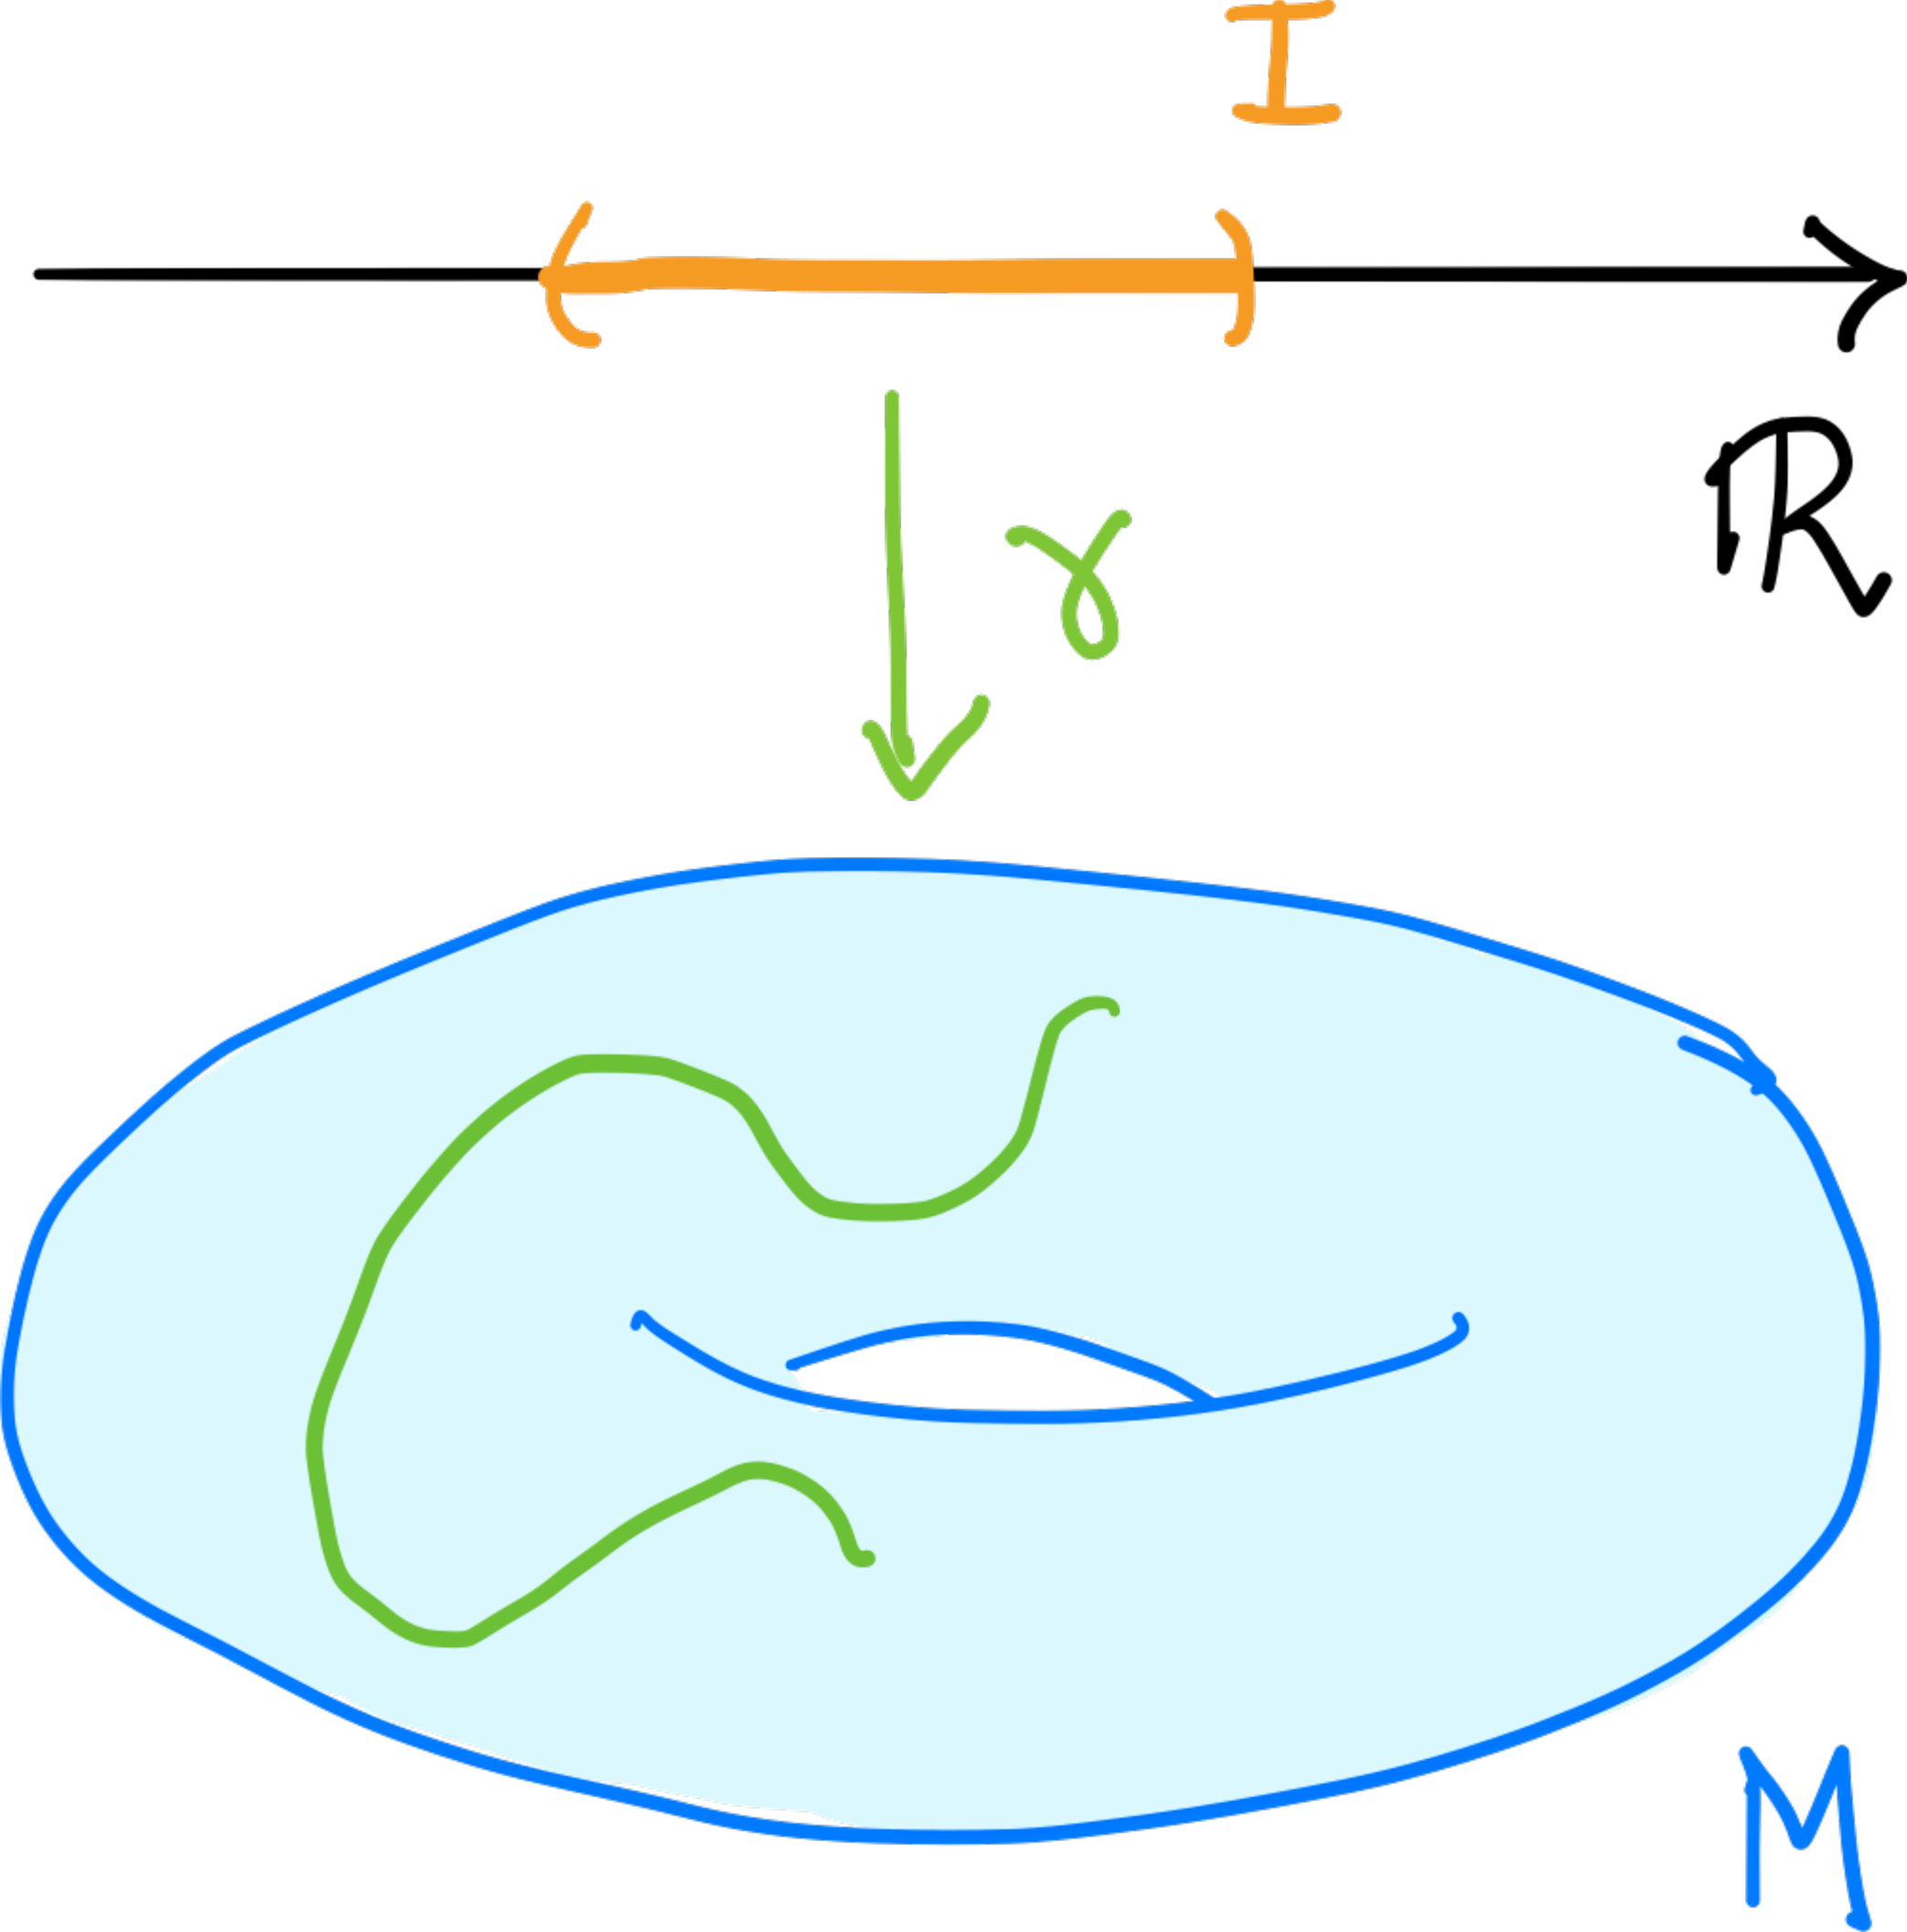
\includegraphics{2_2-curve-on-M.pdf}
\end{marginfigure}

Fix $t\in(a,b)$. 
A priori we have two different ways to define the \emph{velocity vector of $\gamma$ at a time $t$}, that is, an element $\gamma'(t) \in T_{\gamma(t)}M$:
\begin{enumerate}
  \item We can define a derivation on $C^\infty(M)$ at $\gamma(t)$ by setting
  \begin{equation}\label{eq:tg_curve_der}
    \gamma'(t) (f) := (f\circ\gamma)'(t), \quad f\in C^\infty(M).
  \end{equation}
  \begin{exercise}
    Show that this is indeed a derivation on $C^\infty(M)$.
  \end{exercise}
  \item If we think of $\gamma$ as a smooth map between manifolds, we can define the tangent vector via the differential $d\gamma_t$:
  \begin{equation}\label{eq:tg_curve_diff}
    \gamma'(t):= d\gamma_t\left(\frac{\partial}{\partial t}\Big|_t\right) \in T_{\gamma(t)}M.
  \end{equation}
\end{enumerate}

Do these definition agree?
One way to check is to pick a chart $\phi: U \to \phi(U)$ in a neighborhood of $gamma(t)$, and compare the expressions in local coordinates. Let $(x^i)$ denote the coordinates of $\phi$ and define the curves $\gamma^i := x^i \circ \gamma : I\to\R$.
Let's focus on \eqref{eq:tg_curve_der}. By definition, $\gamma'(t)(x^i) = (x^i\circ\gamma)'(t) = (\gamma^i)'(t)$, therefore by Proposition~\ref{prop:basis_TpM} we get
\begin{equation}\label{eq:tg_curve_vec}
  \gamma'(t) = %\sum_{i=1}^m
    \gamma'(t)(x^i) \frac{\partial}{\partial x^i}\Big|_\gamma(t).
\end{equation}
\begin{exercise}
  Show that applying Proposition~\ref{prop:DiffCoords} to \eqref{eq:tg_curve_diff} leads to the same formula as \eqref{eq:tg_curve_vec}.
\end{exercise}

\begin{figure*}[htp]
  \centering
  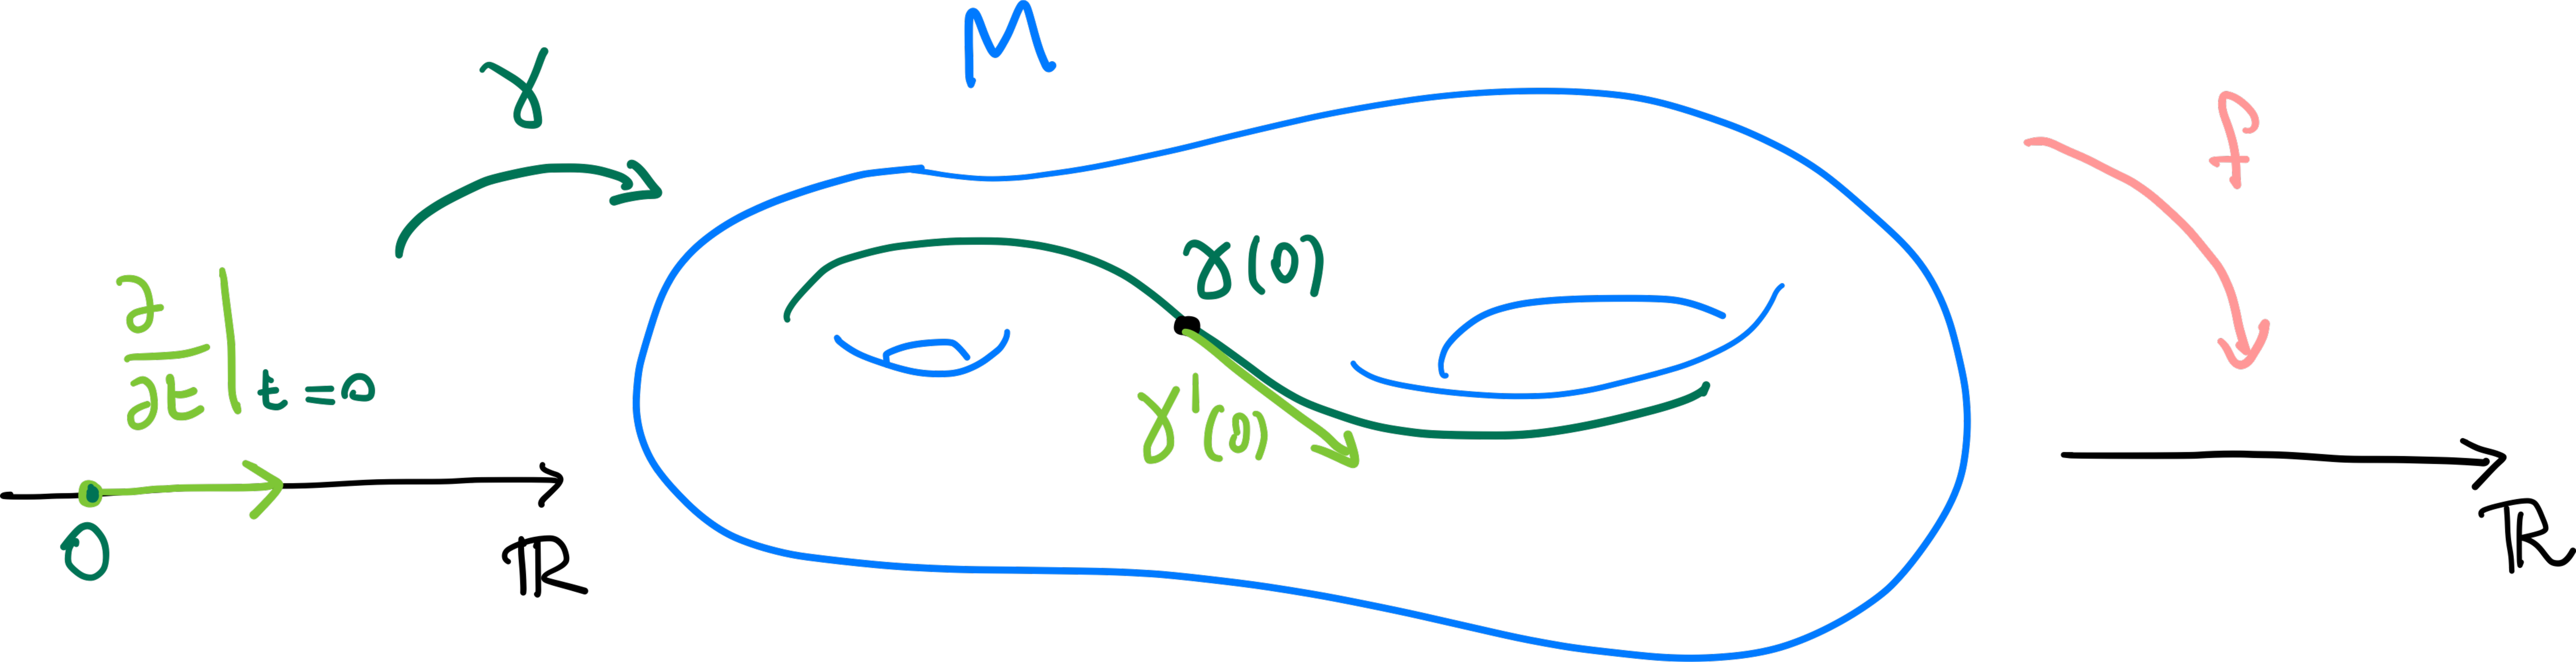
\includegraphics{2_5-v_cur_full.pdf}
  \caption{The velocity of a curve}
  \label{fig:2_5-v_cur_full}
\end{figure*}

But how can this be well defined? Surely, there must be multiple curves with the same speed at a point which differ outside a neighborhood of the point.

\begin{lemma}\label{lem:equiv_tg_curves}
  Let $M$ be a smooth manifolds and $\gamma, \delta : (-\epsilon, \epsilon) \to M$ two smooth curves with $\gamma(0) = \delta(0)$. Then, $\gamma'(0) = \delta'(0)$ as elements of $T_{\gamma(0)}M$ if and only if for some (and thus any) chart $\phi:U\to\phi(U)$, $\gamma(0)\in U$, we have $(\phi\circ \gamma)'(0) = (\phi\circ\delta)'(0)$.
\end{lemma}
\begin{proof}
  Let $(x^i)$ denote the coordinates of $\phi$. The condition $(\phi\circ \gamma)'(0) = (\phi\circ\delta)'(0)$ is equivalent as stating that $(\gamma^i)'(0) = (\delta^i)'(0)$, where $\gamma^i = x^i\circ\gamma$ and $\delta^i=x^i\circ\delta$. Then, the claim follows from \eqref{eq:tg_curve_vec} and the fact that $\left\{\frac{\partial}{\partial x^i}\big|_{\gamma(0)}\right\}$ is a basis of $T_{\gamma(0)}M$.
\end{proof}

This seems to follow a pattern: until now, all the definitions of tangent vectors where in terms of classes of equivalence.
There is still a potential problem, though. We don't yet know if \emph{every} tangent vector can be written as the velocity vector of a curve.

\begin{theorem}
  Let $M$ be a smooth $n$-manifold, let $p\in M$ and let $v\in T_pM$.
  There exists a smooth curve $\gamma: (-\epsilon,\epsilon) \to M$ such that $\gamma'(0) = v$.
\end{theorem}
\begin{proof}
  Let $\phi:U\to\phi(U)$ be a chart about $p$ such that $\phi(p)=0$.
  Let $(x^i)$ denote the coordinates of $\phi$, as usual, and assume that
  \begin{equation}
    v = \sum_{i=1}^n a^i \frac{\partial}{\partial x^i}\Big|_p, \qquad a^i \in\R.
  \end{equation}
  For $\epsilon$ small enough, by continuity the vector $(ta^1, \ldots, ta^n) \in \phi(U)$ for all $|t|<\epsilon$. Therefore, the curve
  \begin{equation}
    \gamma: (-\epsilon, \epsilon) \to M, \quad \gamma(t):=\phi^{-1}(ta^1, \ldots, ta^n),
  \end{equation}
  is well-defined, smooth, satisfies $\gamma(0) = p$ and, by \eqref{eq:tg_curve_vec}, $\gamma'(0) = v$.
\end{proof}

\begin{marginfigure}
  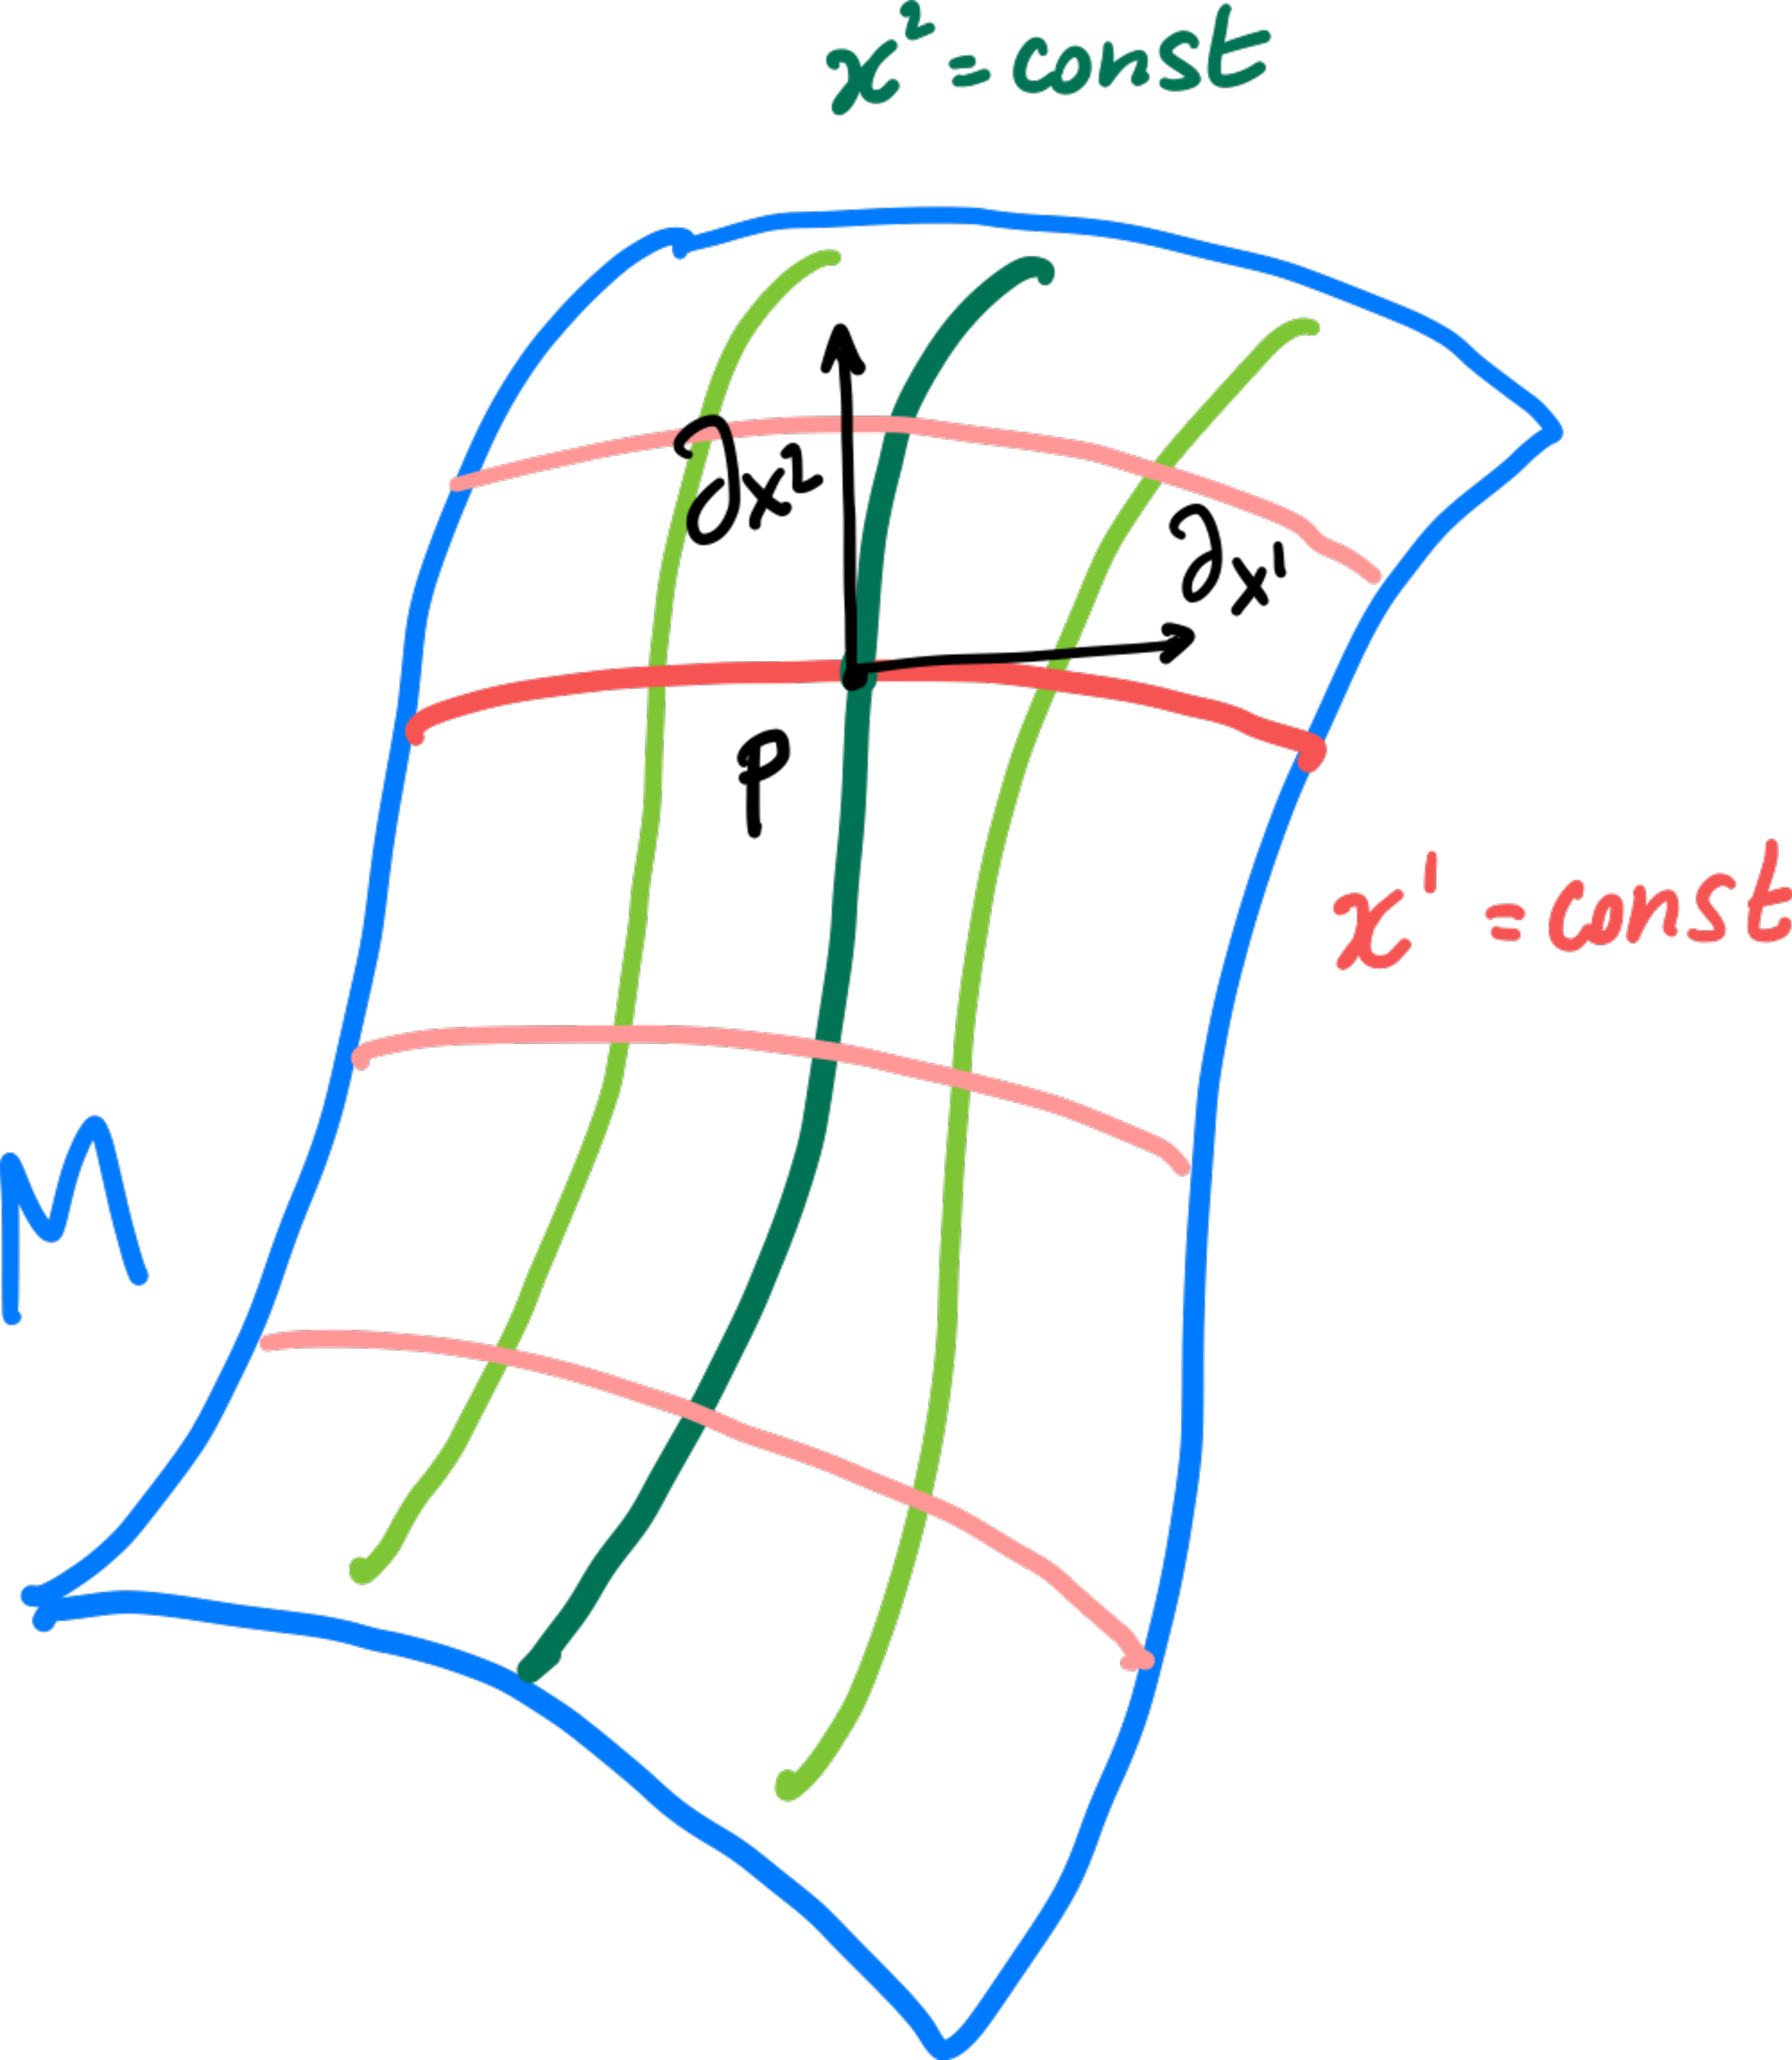
\includegraphics{2_4-v_cur.pdf}
  \caption{With this definition, the coordinate tangent vectors $\partial_{x^i}\in T_p M$ become the tangent vectors defined by the curve \[t \mapsto \phi^{-1}(x^1(p), \ldots, {x^i(p) + t}, \ldots, x^n(p)).\]}
  \label{fig:2_4-v_cur}
\end{marginfigure}
This means that we can actually make an alternative definition of $T_xM$ in terms of tangent to curves:
\begin{quote}
  a tangent vector at $p\in M$ is an equivalence class of smooth curves $\gamma:(-\epsilon, \epsilon)\to M$ such that $\gamma(0)=p$, where $\gamma\sim\delta$ if and only if $(\phi\circ \gamma)'(0) = (\phi\circ\delta)'(0)$ for some chart centered about $p$ (see Lemma~\ref{lem:equiv_tg_curves}).
\end{quote}

In fact, it is possible to start the whole tangent space discussion with the above definition. In that case, you would first need to prove Exercise~\ref{exe:vsstruct} and to endow $T_xM$ with a vector space structure\footnote{To get the analogue result as Proposition~\ref{prop:basis_TpM}}.

To conclude this part, the next proposition shows that velocity vectors behave well under composition with smooth maps and gives us direct, explicit and effective way to compute differentials.

\begin{proposition}\label{prop:curves_deriv}
  Let $F:M\to N$ b a smooth map between smooth manifolds and $\gamma:I\to M$ a smooth curve in $M$.
  Then
  \begin{equation}
    d F_{\phi(t)} (\phi'(t)) = (F\circ\gamma)'(t).
  \end{equation}
\end{proposition}
\begin{proof}
  We are going to use \eqref{eq:tg_curve_diff} as definition of $\gamma'(t)$.
  Applying the chain rule we obtain:
  \begin{align}
    d F_{\phi(t)} (\phi'(t))
    &= d F_{\phi(t)} \circ d\phi_t \left(\frac{\partial}{\partial t}\Big|_t\right) \\
    &= d (F\circ\gamma)_t \left(\frac{\partial}{\partial t}\Big|_t\right) \\
    &= (F\circ\gamma)'(t).
  \end{align}
\end{proof}

\begin{exercise}
  Give an alternative proof of Proposition~\ref{prop:curves_deriv} using \eqref{eq:tg_curve_der} as definition for $\gamma'(t)$.
  Hint: use the definitions to rewrite the formula in different ways.
\end{exercise}

\section{The tangent bundle}

Instead of working separately with the various tangent spaces, we can ``glue'' them together into a big manifold.

\begin{marginfigure}
  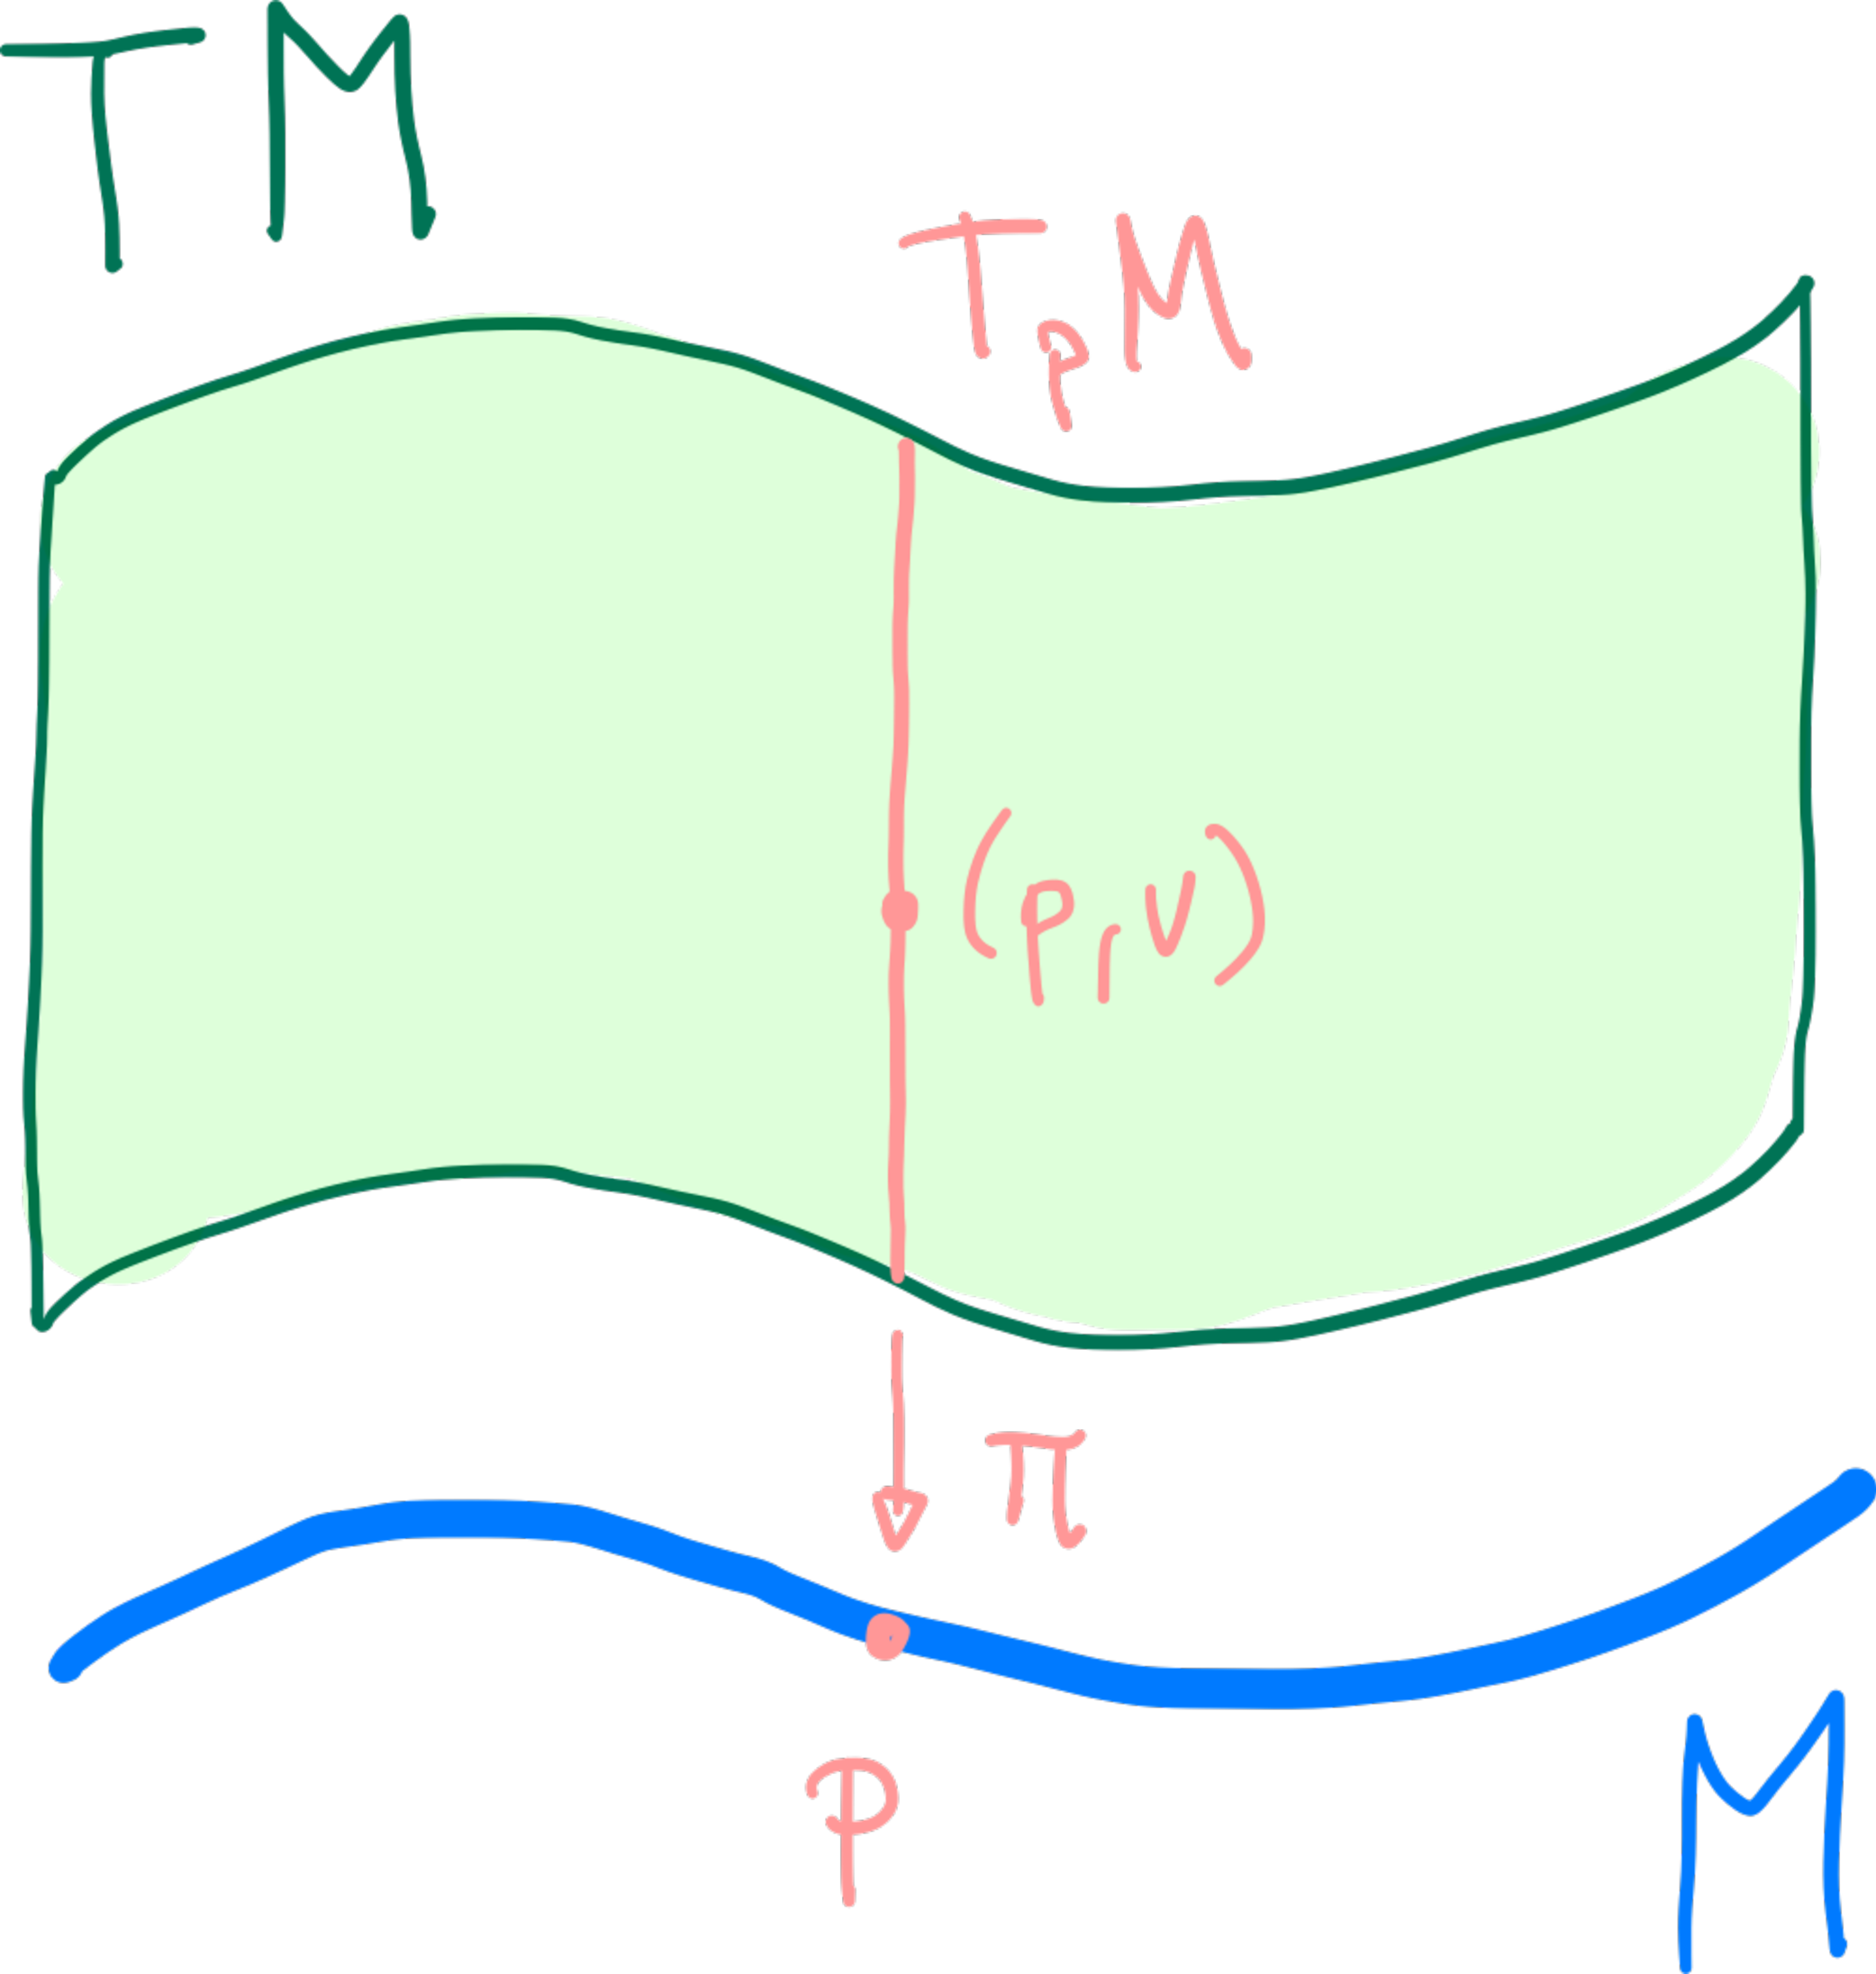
\includegraphics{2_6-tg_bdl_proj.pdf}
\end{marginfigure}
\begin{definition}
  The \emph{tangent bundle} $TM$ of $M$ is the disjoint union of the tangent spaces
  \begin{equation}
    TM := \bigsqcup_{p\in M}\left(\{p\}\times T_pM\right)
       = \{(p,v) \;\mid\; p\in M,\, v\in T_pM\}.
  \end{equation}  
\end{definition}

Elements in $TM$ are pairs\sidenote[][1.5em]{We will often abuse notation and identify $T_pM$ with with its image under the canonical injection $v\mapsto(p,v)$ and use interchangeably any of the notations $v$, $v_p$ or $(p,v)$ for a vector in $T_pM$ (depending on how much emphasis we need to put on the base point).} $(p,v)$ of a \emph{base point} $p\in M$ and a \emph{tangent vector} $v\in T_pM$.

To the tangent bundle we associate a surjective map $\pi:TM \to M$, the \emph{projection (onto the base)}, which sends each vector in a tangent space to the point at which it is tangent, that is, $\pi(p,v) = p$.
The second component of the pre-image $\pi^{-1}(\{p\}) = \{p\}\times T_pM$ is called the \emph{fibre} over $p\in M$.
We will come back to this later on once we talk about vector bundles.

\begin{example}
  Let $M\subset \R^n$ be an an open set.
  We can identify $TM$ in a natural way with $M\times\R^n$.
  Since $M\times\R^n \subset \R^{2n}$ and thus is a manifold, we can equip the tangent bundle $TM$ with the structure of a manifold induced by this identification.
\end{example}

As it turns out, this is a particular instance of a more general fact.

\begin{theorem}
  Let $M$ be a smooth $n$-manifold.
  The smooth structure on $M$ naturally induces a smooth structure on $TM$, making $TM$ into a smooth manifold of dimension $2n$.
  Moreover, the map $\pi: TM \to M$ is smooth.
\end{theorem}
\begin{proof}
  \marginnote[1em]{In this proof you can see instances of a typical abuse of notation: in the expressions $\tilde x^i(x)$ we think of the $\tilde x^i$ as coordinate functions but we think of the $x$ as representing a point in $\phi(U\cap V)$.}
  \newthought{Step 1: extending charts from $M$ to $TM$.}
  Given a chart $(U,\phi)$ about $p\in M$, the preimage $\phi^{-1}(U) \subset TM$ is the set of all tangent vectors to $M$ at points of $U$.
  If $(x^i)$ denotes the coordinate functions of $\phi$, we can define a map $\tilde\phi : \pi^{-1}(U) \to \phi(U)\times\R^n \subset \R^{2n}$ by
  \begin{align}\label{eq:nat_coords}
    \tilde\phi\left(v^i \frac{\partial}{\partial x^i}\Big|_p\right) := \left(x^1(p), \ldots, x^n(p), v^1, \ldots, v^n\right).
  \end{align}
  Since $\tilde\phi$ can be explicitly inverted as $\tilde\phi^{-1}\left(v^i \frac{\partial}{\partial x^i}\Big|_p\right) = v^i \frac{\partial}{\partial x^i}\Big|_{\phi^{-1}(x)}$, it defines a bijection onto it image.

  \newthought{Step2: compatibility of the extended charts.}
  Suppose we have two smooth charts $(U,\phi)$, $(V,\psi)$ for $M$.
  Let $(\pi^{-1}(U),\tilde\phi)$, $(\pi^{-1}(V),\tilde\psi)$ be their extension\footnote{These are called \emph{bundle charts}.} to $TM$ as in the previous step.
  By construction, both $\tilde\phi(\pi^{-1}(U)\cap\pi^{-1}(V)) = \phi(U\cap V)\times\R^n$ and $\tilde\psi(\pi^{-1}(U)\cap\pi^{-1}(V)) = \psi(U\cap V)\times\R^n$ are open in $\R^{2n}$.
  Moreover, we can take advantage of Remark~\ref{rmk:chg_coords} to write explicitly the transition map  $\tilde\psi\circ\tilde\phi^{-1}: \phi(U\cap V)\times\R^n \to \psi(U\cap V)\times\R^n$ as
  \begin{align}
    \tilde\psi\circ&\tilde\phi^{-1}\left(x^1, \ldots, x^n, v^1, \ldots, v^n\right) \\
    &=\left(\tilde x^1(x),\ldots, \tilde x^n(x), \frac{\partial \tilde x^1}{\partial x^j}(x) v^j, \ldots, \frac{\partial \tilde x^n}{\partial x^j}(x) v^j\right)
  \end{align}
  Which is clearly smooth.

  \begin{figure*}[htp]
    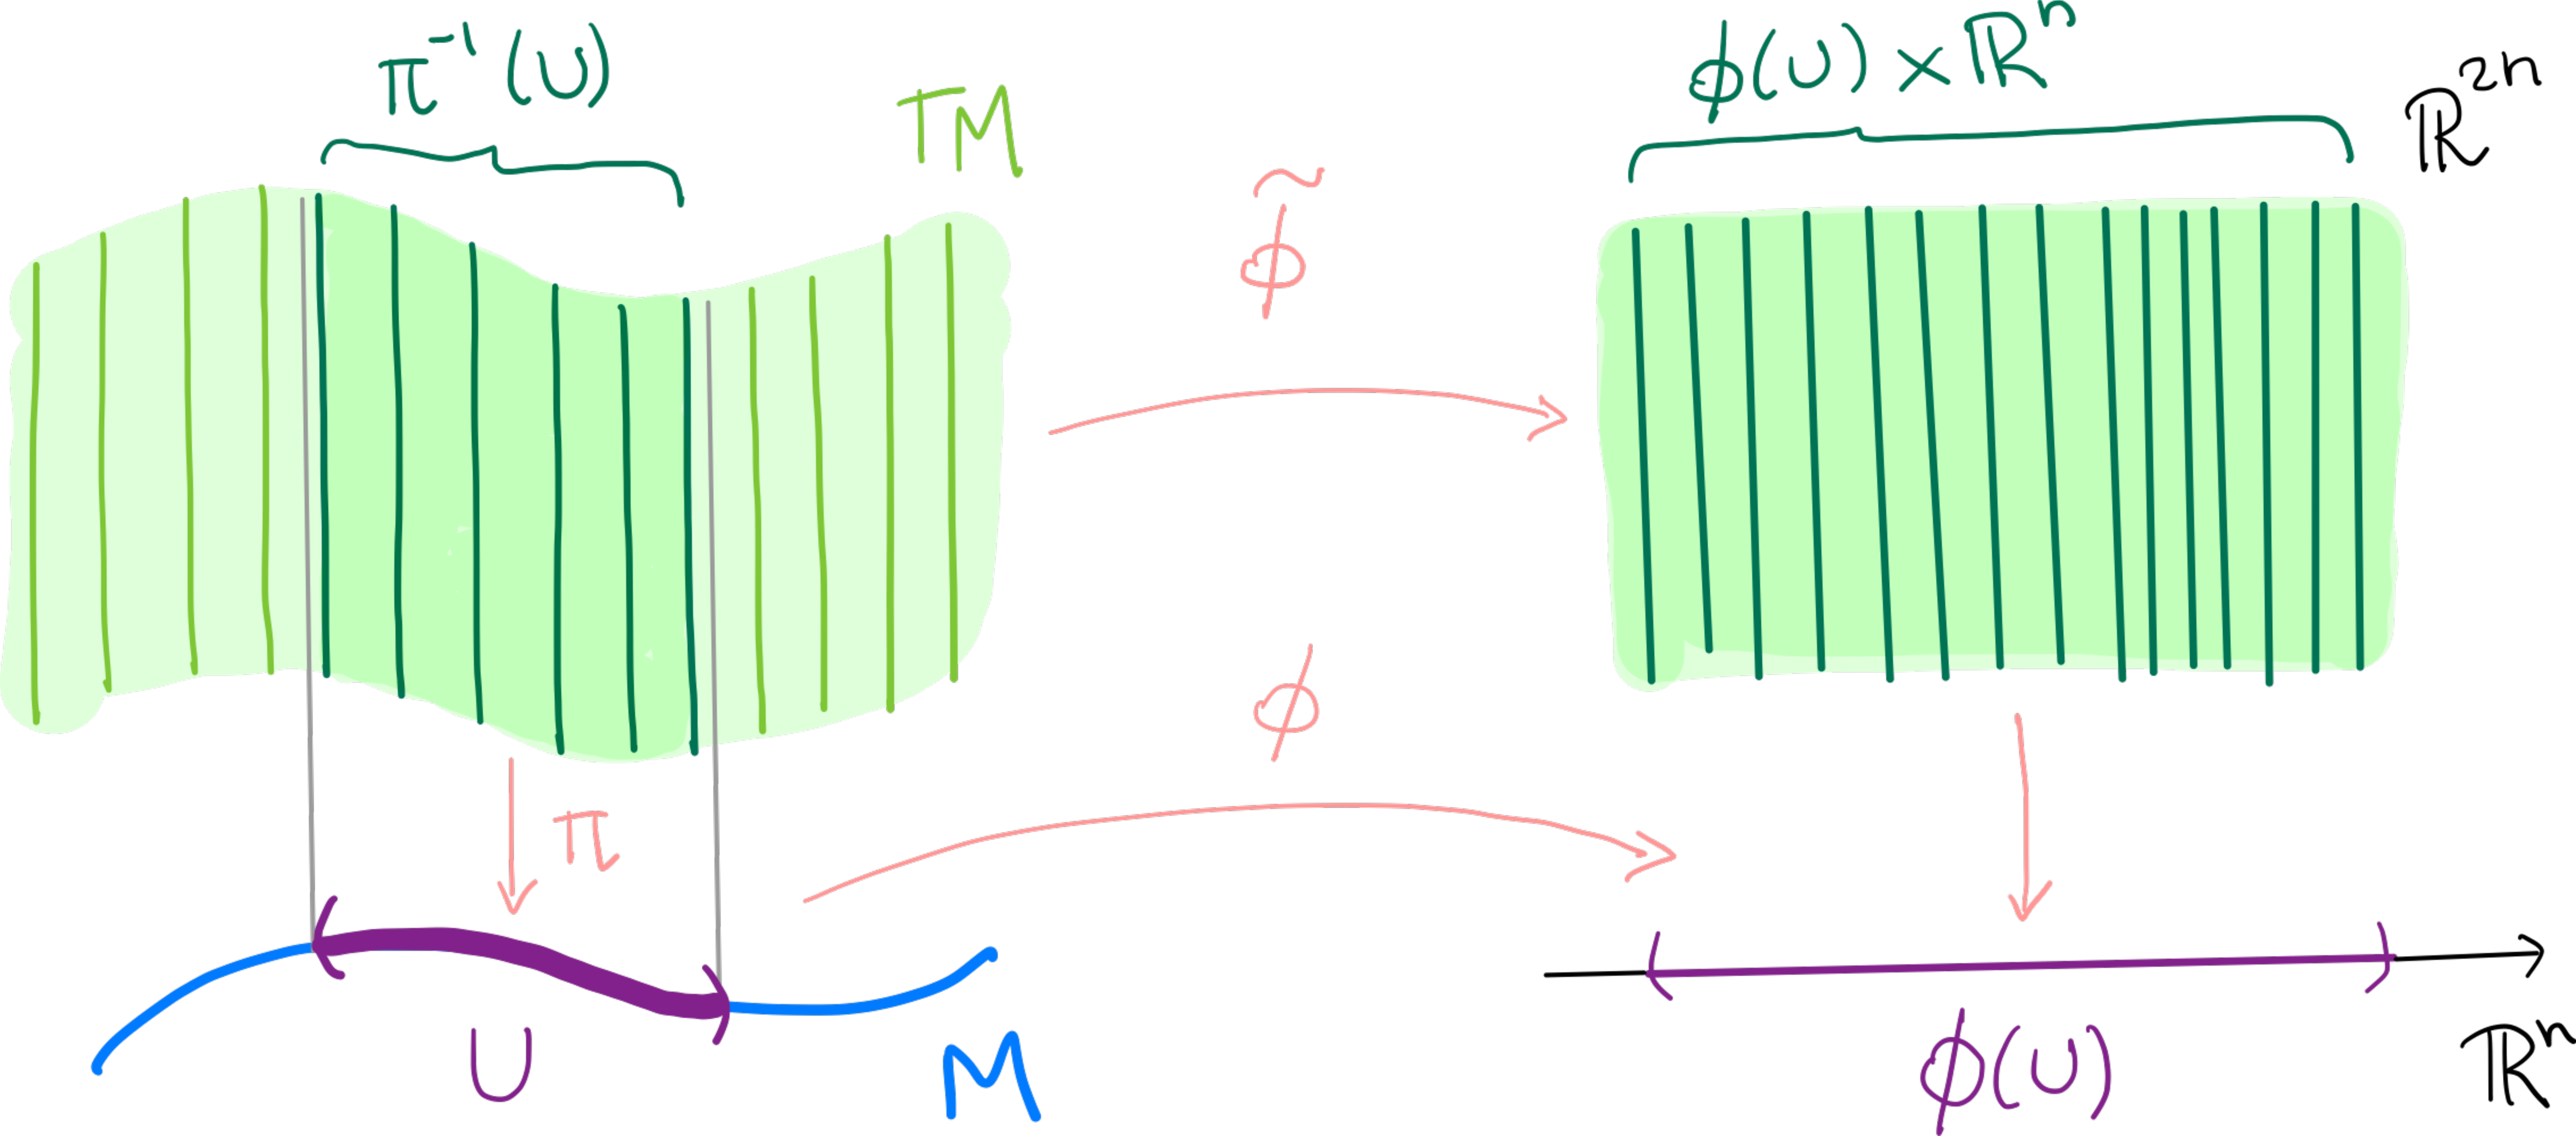
\includegraphics{2_7-tg_bdl_coord.pdf}
    \caption{Coordinates for the tangent bundle}
  \end{figure*}
  
  \newthought{Step3: $TM$ is a manifold.}
  With the procedure delineated above, a countable smooth atlas $\{(U_i, \phi_i)\}$ of $M$ induces a countable atlas $\{(\pi^{-1}(U_i), \tilde\phi_i)\}$ of $TM$.
  First of all, $\{(\pi^{-1}(U_i)\}$ provides a countable covering of $TM$.
  
  We only need to show that the topology induced by the charts is Hausdorff and second countable.
  
  Let $(p^1, v^1), (p^2, v^2) \in TM$ be different points: either $p^1\neq p^2$, or $p^1 = p^2$ and $v^1 \neq v^2$.
  In the first case, there are disjoint open sets $V_1, V_2 \subset U_i$ (for some $i$) containing respectively $p^1$ and $p^2$.
  Then $\tilde\phi_i^{-1}(V_1\times\R^n)$ and $\tilde\phi_i^{-1}(V_2\times\R^n)$ are disjoint open sets containing respectively $(p^1, v^1)$ and $(p^2, v^2)$.
  In the second case, $p=p^1=p^2$ there are disjoint open sets $V_1,V_2\subset \R^n$ containing $v^1$ and $v^2$ respectively.
  Again the preimages $\tilde\phi^{-1}(U_i\times V_1)$ and $\tilde\phi^{-1}(U_i\times V_2)$ (for some $i$) are disjoint open sets containing respectively $(p^1, v^1)$ and $(p^2, v^2)$.

  If countable basis $\{U_j\}$ is countable basis for the topology of $M$ (which is second countable) and $\{W_k\}$ is a countable basis for the topology of $\R^n$, then $\{\tilde\phi^{-1}((U_i\cap U_j)\times W_k)\}$ is a countable basis for $TM$.
  The charts defined above make $TM$ automatically euclidean of dimension $2n$.

  \begin{exercise}
    This part of the proof seems unnecessarily detailed.
    Can you simplify it using Lemma~\ref{lem:manifold_chart}?
  \end{exercise}

  \newthought{Step4: $\pi$ is smooth.} With respect to the charts $(U,\phi)$ for $M$ and $(\pi^{-1}(U), \tilde\phi)$ for $TM$, the coordinate representation of $\pi$ is $\pi(x,v) = x$.
\end{proof}

The coordinates $(x^i, v^i)$ defined by \eqref{eq:nat_coords} are called \emph{natural coordinates}.

\begin{exercise}
  Show that the differential of a smooth map is a smooth map between manifolds. Hint: use the natural differentiable structure on the tangent bundle described above and the definition of smooth map.
\end{exercise}

Even though \emph{locally} $TM$ is diffeomorphic to $M\times\R^n$, this is not true in general with one exception.

\begin{exercise}
  Let $M$ be a smooth $n$-manifold that can be covered by a single smooth chart. Then $TM$ is diffeomorphic to $M\times\R^n$. In this case the bundle $TM$ is called \emph{trivialisable} (and its base $M$ is called \emph{parallelisable}).
\end{exercise}

\begin{remark}
  In classical mechanics, the configuration space is usually a manifold $M$.
  The tangent bundle $TM$ corresponds to the state space, that is, the space of configurations and velocities. In symbols $x=(q,v)$ is a pair of a configuration $q = \pi(x)$ and a velocity $v\in T_q M$.
  It turns out that the Lagrangian is a function on $TM$.
\end{remark}

\section{Submanifolds}

With differentials of smooth functions at hand, we are ready to discuss submanifolds: smaller manifolds sitting inside larger ones.

\begin{definition}
  Let $M^m$ and $N^n$ be differentiable manifolds and $F:M\to N$ a $C^1$ function.
  \begin{enumerate}
    \item $F$ is an \emph{immersion} if $dF_p$ is injective for all $p\in M$ ($\Rightarrow\; m\leq n$);
    \item $F$ is a \emph{submersion} if $dF_p$ is surjective for all $p\in M$ ($\Rightarrow\; m\geq n$);
    \item $F$ is an \emph{embedding} if $F$ is an injective immersion that is also a homeomorphism onto its range $F(M)\subset N$.
  \end{enumerate}
\end{definition}

\begin{example}
  \begin{enumerate}
    \item The prototype of an immersion is the inclusion of $\R^m$ in a higher-dimensional $\R^n$:
    \begin{align}
      i &: \R^m \hookrightarrow \R^n,\\
      i &: \left(x^1, \ldots, x^m\right) \mapsto \left(x^1, \ldots, x^m, \LaTeXunderbrace{0, \ldots, 0}_{m-n}\right).
    \end{align}
    
    Indeed, the $n\times m$ matrix
    \begin{equation}
      di_x = Di(x)
       = \begin{pmatrix}
        1 & 0 & \cdots & 0 \\
        0 & 1 & \cdots & 0 \\
        \vdots & & \ddots & \vdots \\
        0 & \cdots & \cdots & 1 \\
        0 & \cdots & \cdots & 0 \\
        \vdots & & & \vdots \\
        0 & \cdots & \cdots & 0
       \end{pmatrix}
    \end{equation}
    has full rank (equal to $m$) and is therefore injective.
    Moreover, the map $i$ is injective and continuously invertible on its range, so it is also an embedding.

    \item The prototype for a submersion is the projection of $\R^m$ onto a lower-dimensional $\R^n$: $\pi\left(x^1,\ldots,x^m,x^{m+1},\ldots,x^n\right) = \left(x^1,\ldots,x^m\right)$.
    
    Indeed, the $m\times n$ matrix
    \begin{equation}
      d\pi_x = D\pi(x)
       = \begin{pmatrix}
        1 & 0 & \cdots & 0 & 0 & \cdots & 0 \\
        0 & 1 & \cdots & 0 & \vdots & & \vdots \\
        \vdots & & \ddots & \vdots & \vdots & & \vdots \\
        0 & \cdots & \cdots & 1 & 0 & \cdots & 0
       \end{pmatrix}
    \end{equation}
    has full rank (equal to $n$) and is therefore surjective.
    Hence, $i$ is a submersion.

    \item Let $n=1$, $m > 1$ and $\gamma:\R\to\R^m$ a smooth curve.
    The map $\gamma$ is an immersion if and only if its velocity vector satisfies $\gamma'(t)\neq0$ for all $t\in\R$.
    If the curve intersects itself, e.g $f(t_1) = f(t_2)$ for some $t_1\neq t_2$, then $f$ is not an embedding.
  \end{enumerate}
\end{example}

\begin{remark}
  Surjectivity of submersions or injectivity of immersions are properties of the differentials, not of the maps themselves.
  
  For example, if $U\subset M$ open, the inclusion $i: U \to M$ is both an immersion and a submersion.
\end{remark}

\begin{definition}
  Let $M$ an $N$ smooth manifolds such that $M\subset N$ as a set.
  We say that $M$ is an \emph{embedded submanifold} of $N$ if the inclusion $M\hookrightarrow N$ is an embedding. If the inclusion is just an immersion, we say that $M$ is an \emph{immersed submanifold}.
\end{definition}

Before moving on, it is useful to recall some results from multivariable analysis.
A function $f:\R^m \to \R^n$ between euclidean spaces has rank $k$ at $x\in\R^m$ if its ($n\times m$) Jacobian matrix $Df(x)$ has rank $k$.
The function has maximal rank at $x$ if $k = \min(n,m)$.
When $n=m$, $f$ has maximal rank at $x$ if and only if the square matrix $DF(x)$ is an invertible matrix.

As for many local properties, this definition carries over to manifolds rather ``smoothly''.

\begin{definition}
  A smooth map $F:M\to N$ has \emph{rank $k$} at a point $p$ if the linear subspace $dF_p(T_pM)$ has dimension $k$ inside $T_{F(p)}N$.
\end{definition}

And the same is true for the inverse function theorem:
compare the following statements.

\begin{theorem}[Inverse function theorem]\label{thm:ift}
  Let $U\subset\R^m$ open and $f:U \to \R^n$ be a smooth map.
  Assume that $f$ has maximal rank at some $x\in U$, then there exists a neighborhood $\Omega\subset U$ of $x$ such that  $f\big|_\Omega : \Omega \to f(\Omega)$ is a diffeomorphism.
\end{theorem}

\begin{theorem}[Inverse function theorem for manifolds]\label{thm:iftm}
  Let $F:M\to N$ be a smooth function between manifolds of the same dimension $n$.
  Let $p\in M$ and assume that $F$ has maximal rank (i.e. rank $n$) at $p$.
  Then there exists a neighborhood $V$ of $p$ such that the restriction $F:V\to F(V)$ is a diffeomorphism.
\end{theorem}
% \begin{proof}
%   This is a purely local statement.
%   Let $(U,\phi)$ be a chart about $p\in M$ and let $(V, \psi)$ be a chart about $F(p)\in N$.
%   Since both $\phi$ and $\psi$ are diffeomorphisms (and thus have maximal rank), the derivative of
%   \begin{equation}
%     \psi \circ F \circ \phi^{-1}: \phi(U\cap F^{-1}(V)) \to \psi(F(U)\cap V)
%   \end{equation}
%   has rank $n$ at $\phi(p)$.
%   Thus the inverse function theorem, Theorem~\ref{thm:ift}, there exists $\Omega \subset \phi(U\cap F^{-1}(V))$ such that $\psi \circ F \circ \phi^{-1}\big|_{\Omega}$ is a diffeomorphism.
%   Therefore, once again since both $\phi$ and $\psi$ are diffeomorphisms, $F\big|_W : W \to F(W)$ is also a diffeomorphism for $W := \phi^{-1}(\Omega)$.
% \end{proof}
\begin{exercise}
  Use the euclidean inverse function theorem\footnote{Theorem~\ref{thm:ift}.} on $\R^n$ to prove Theorem~\ref{thm:iftm}.
\end{exercise}


In fact, also analogues of the implicit functions theorem carry over.
We will state them without going into the details of the proofs.

\begin{proposition}\label{prop:slice_chart}
  Let $F:M^m\to N^n$ be an immersion.
  Then for any $p\in M$, there exists a neighborhood $U$ of $p$ and a chart $(V,\psi)$ about $F(p)\in N$ such that
  \begin{enumerate}
    \item If $y^i = r^i\circ \psi$ are the local coordinates of $\psi$ then
    \begin{equation}\label{eq:slice_chart}
      F(U)\cap V = \left\{ q \in V \;\mid\; y^{m+1}(q)=\cdots=y^n(q)=0\right\};
    \end{equation}
    \item $F\big|_U$ is an embedding.
  \end{enumerate}
 \end{proposition}

If $F$ is an embedding, and this $M$ is an embedded submanifold, then the set $F(U)$ above can be written as $F(U) = F(M)\cap W$ for some open set $W\subset N$.
By replacing $V$ in \eqref{eq:slice_chart} with $V\cap W$, one gets 
\begin{equation}
  F(M)\cap V = \left\{ q \in V \;\mid\; y^{m+1}(q)=\cdots=y^n(q)=0\right\}.
\end{equation}
In particular, this means that a $m$-dimensional submanifold is also a $m$-dimensional manifold whose charts are the ones above after we drop the final $n-m$ components.

The proposition above shows that an immersion is always a local embedding.
\begin{exercise}
  \begin{enumerate}
    \item If $M$ is compact, an injective immersion $F:M\to N$ is always an embedding.
    \item This is not necessarily the case in the non-compact case, give a counterexample.
  \end{enumerate}
\end{exercise}

\begin{lemma}
  With the notation of Proposition~\ref{prop:slice_chart}, assume that around any point $p\in M$ there is a chart of the form
  \begin{equation}
    M\cap V = \left\{ q \in V \;\mid\; y^{m+1}(q)=\cdots=y^n(q)=0\right\} \subset N.
  \end{equation}
  Then, if we endow $M$ with the subspace topology on $N$, $M$ is a topological manifold of dimension $m$.
  Furthermore, it has a smooth structure that makes it into an embedded submanifold of $N$.
\end{lemma}
\begin{proof}[Sketch]
  Let $\pi: \R^n\to\R^m$ be the projection as in the examples above.
  Let $p\in M$ and let $(V,\psi)$ be a chart with coordinates $(y^i)$ of the form above.
  If we endow $M$ with the subspace topology, then $\sigma:= \pi \circ \psi\big|_{M\cap V}$ is a homeomorphism.
  Repeating this at any point we end up with a collection of maps satisfying the hypotheses of Lemma~\ref{lem:manifold_chart}.
  Thus $M$ is a smooth manifold of dimension $n$ and its topology coincides with the subspace topology.

  Finally, with the inclusion $i:M\hookrightarrow N$ one has that $\psi \circ i\circ \sigma^{-1} (p^1,\ldots,p^n) = (p^1,\ldots,p^n,0,\ldots,0)$ which is smooth.
\end{proof}

Up to this point, the first manifold had the same dimension or was smaller than the second one.
What if it is larger?

\begin{marginfigure}
  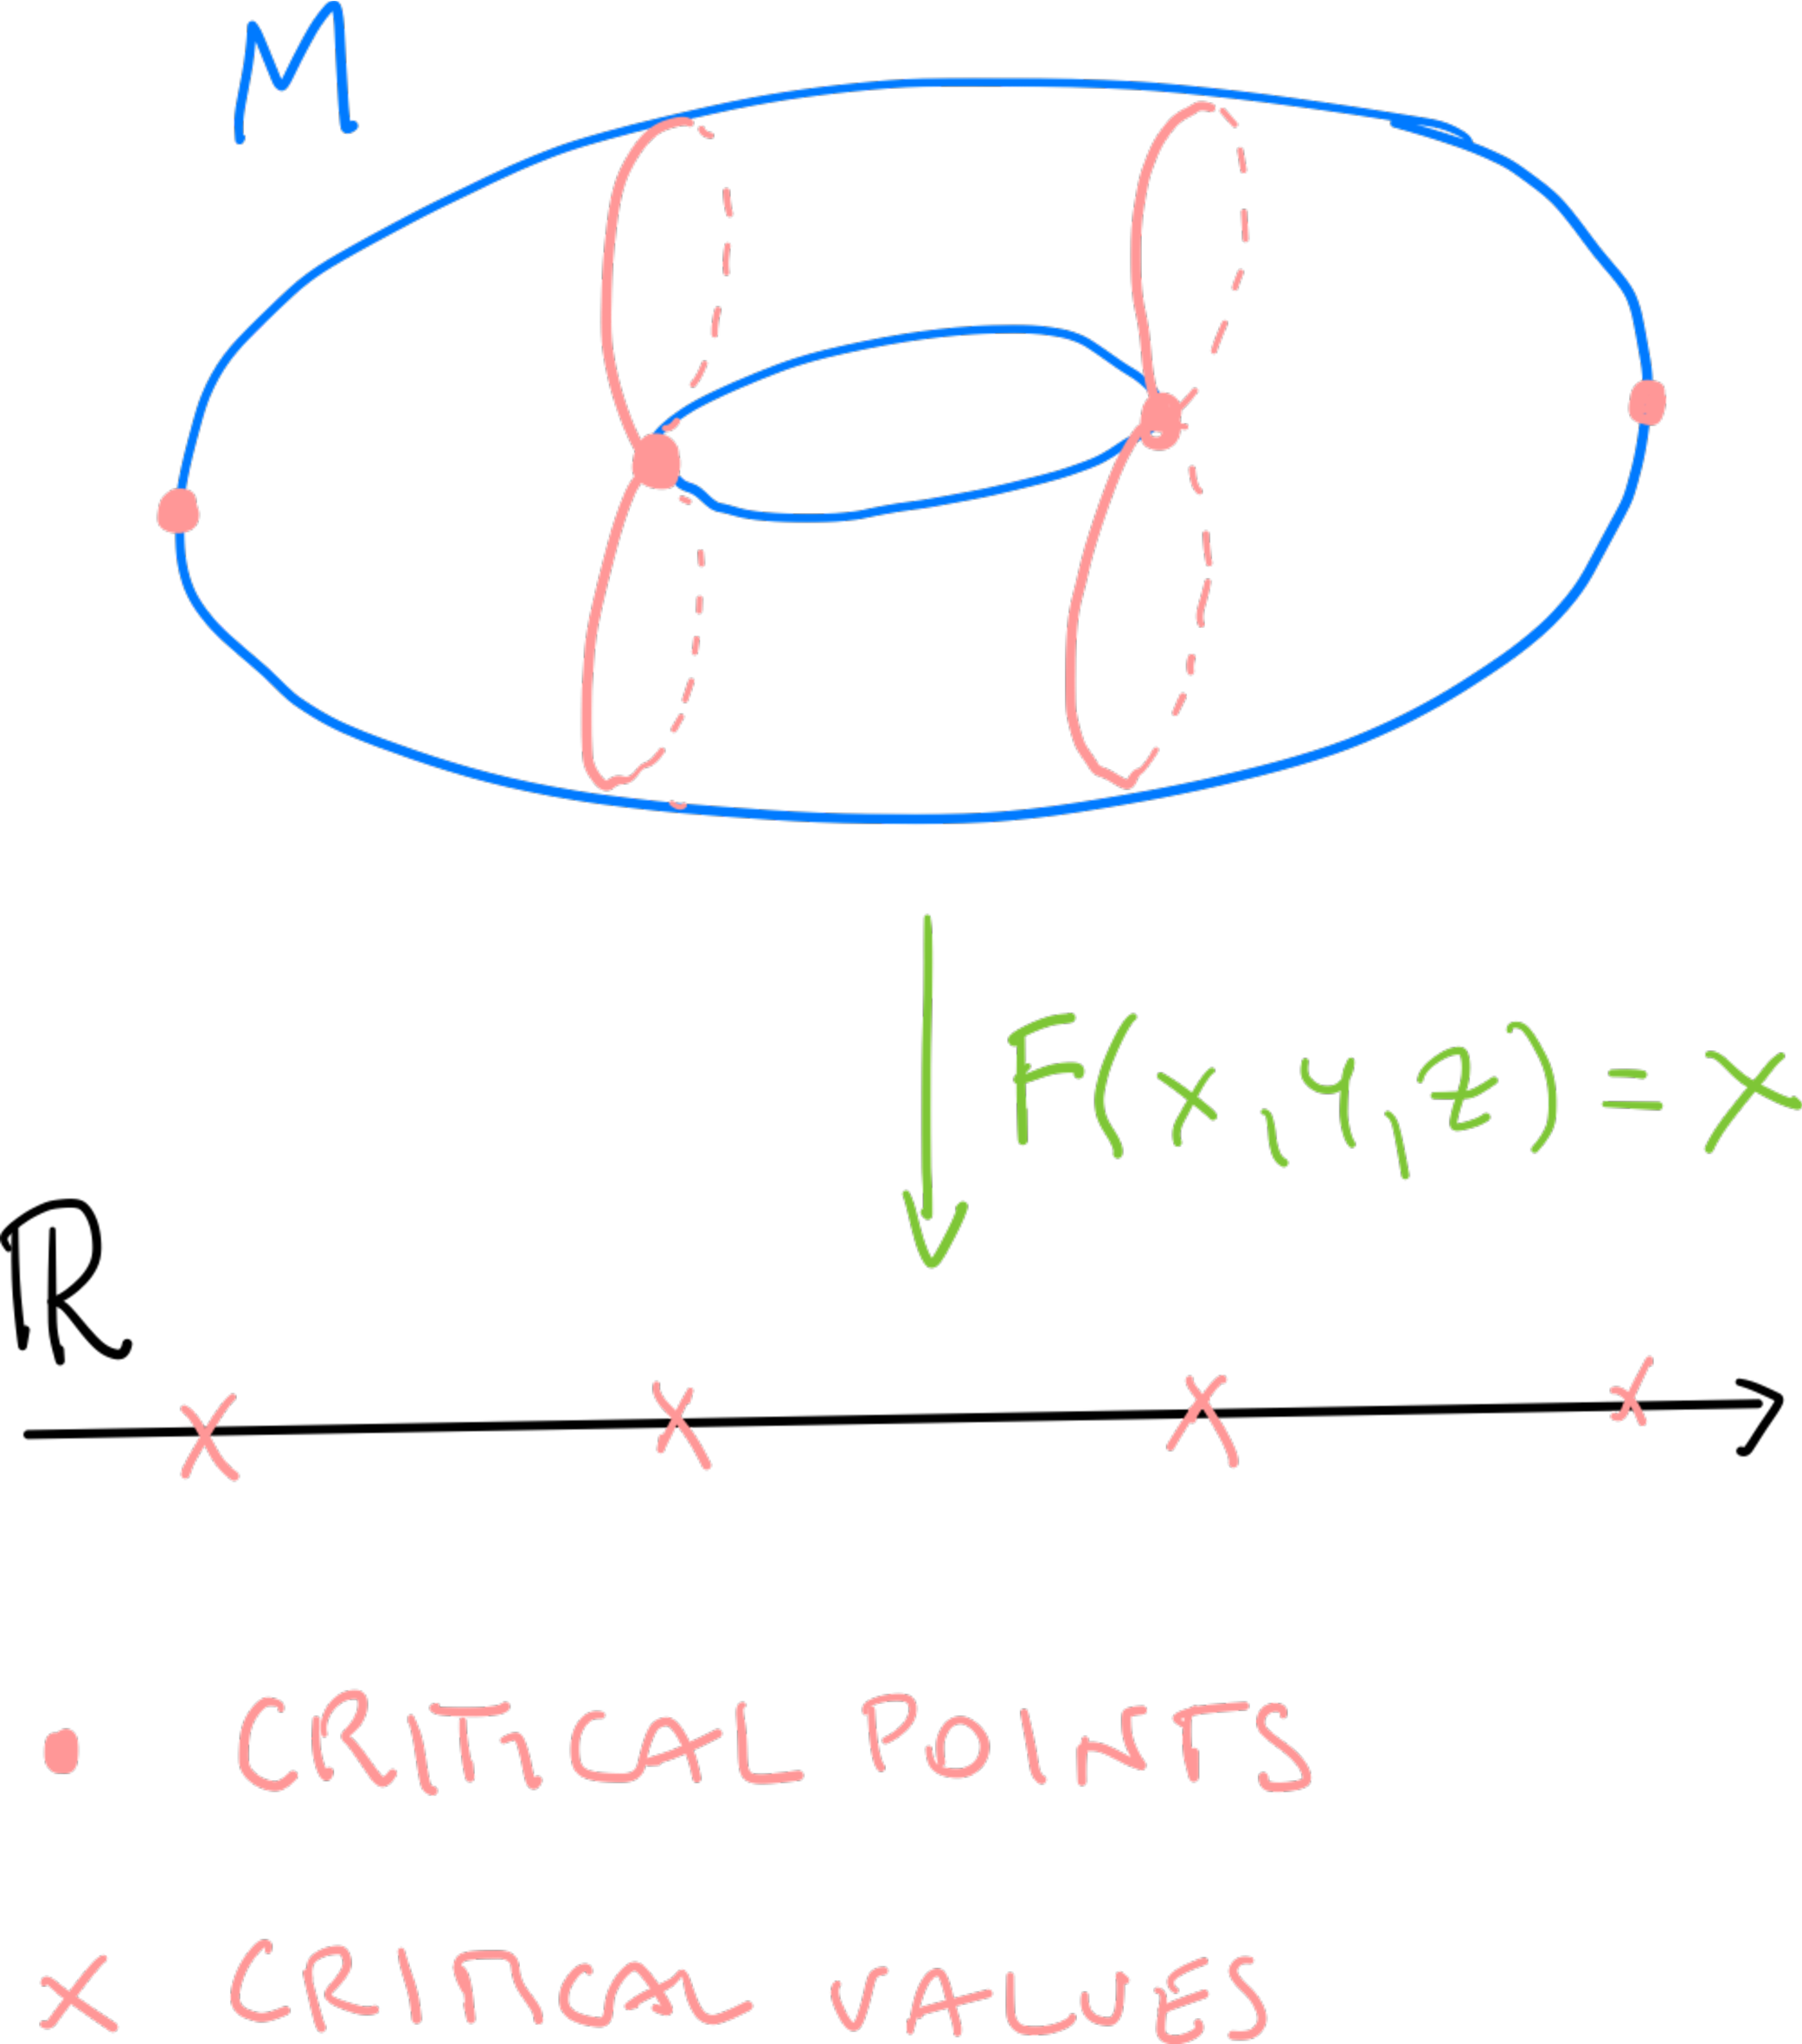
\includegraphics{2_8-crit_pts.pdf}
  \caption{Beware of the subtleties here. The map $F=\pi_x\circ i$ for the inclusion $i:\bT^2\hookrightarrow\R^3$ and the projection $\pi_x(x,y,z)=x$.
  So $dF_p = d (\pi_x)_{i(p)} \circ d i_p$. The latter is zero if $d i_p: T_p\bT^2\hookrightarrow T_p\R^3$ is, which happens when the image of $T_p\bT^2$ is contained in the $yz$-plane (the reason will be clear by the end of the chapter): the critical points depicted here are exactly those points for which the tangent plane is the $yz$-plane.}
\end{marginfigure}
\begin{definition}
  Let $F:M^m \to N^n$ be a smooth map between smooth manifolds.
  A point $p\in M$ is said to be a \emph{regular point} of $F$ if $F$ has rank $n$ at $p$ (which implies that $m\geq n$), while it is called a \emph{critical point} if it is not.

  Similarly, a point $q\in N$ is called a \emph{regular value} if every point in $F^{-1}(q)$ is a regular point, and \emph{critical value} otherwise. If $q\not\in F(M)$, then $q$ is considered a regular value (in the sense that there is nothing to check in its preimage by $F$).
\end{definition}

With this definition at hand, we are ready to state one of the most important theorems in this lecture. Differently from most previous ones, the statement is not local.

\begin{theorem}[Implicit function theorem for manifolds]\label{thm:impl_fun}
  Let $m\geq n$ and let $F: M^m \to N^n$ be a smooth map between smooth manifolds.
  If $q\in N$ is a regular value of $F$ and $P := F^{-1}(q)$ is not empty, then $P$ is a topological manifold of dimension $n-k$. 
  Moreover, there exists a smooth structure on $P$ which makes it into a smooth embedded submanifold of $M$.
\end{theorem}

\begin{remark}
  If $F:M\to N$ is a submersion, Theorem~\ref{thm:impl_fun} implies that any $p\in M$ belongs to the $(n-k)$-dimensional embedded submanifold $F^{-1}(F(p))$.
\end{remark}

From this observation follows another interesting proposition, again consequence of the inverse and the implicit function theorems, of which we will also omit the proof.

\begin{proposition}\label{prop:submanifolds_and_R}
  The following assertions are equivalent.
  \begin{enumerate}
    \item $M^k\subset N^n$ is a $k$-dimensional submanifold.
    \item $M$ is locally the image of an embedding of a subset of $\R^k$. That is, for every $p\in M$ there exists $V\subset M$ open neighborhood of $p$, an open set $U\subset\R^k$ and an embedding
    \begin{equation}
      \phi : U \to N \quad\mbox{such that}\quad \phi(U)=V.
    \end{equation}
    \item $M$ is locally a level set of a submersion into $\R^{n-k}$. That is, for every $p\in M$ there exists $V\subset M$ open neighborhood of $p$ and a submersion $\Phi: V \to\R^{n-k}$ such that
    \begin{equation}
      M\cap V = \{q\in V \;\mid\; \Phi(q) = 0\}.
    \end{equation}
  \end{enumerate}
\end{proposition}

\begin{remark}
  Whitney embedding theorem states that any smooth $n$-dimensional manifold can be smoothly embedded into $\R^{2n}$.
  Thus any abstract manifold is diffeomorphic to a submanifold of $\R^m$ (for some $m$).
\end{remark}

\begin{example}\label{ex:s2}
  The sphere $\bS^2 = \{x\in\R^3 \mid \|x\| = 1\}$ is a $2$-dimensional submanifold of $\R^3$.
  This is immediate using the third condition in the Proposition~\ref{prop:submanifolds_and_R}: let $\Phi(x) = \|x\|^2 -1 : \R^3 \to \R$, then $\Phi$ is smooth, $\bS^2 = \{F(x)=0\}$ and $dF_x(v)= 2x\cdot v \neq 0$ for $x\in\bS^2$.
\end{example}

\begin{example}
  Let $N = \R^2$ and $M = \{ x\in M \;\mid\; x^2 = |x^1| \}$.
  Then $M$ is \emph{not} a submanifold, but it can be equipped with a manifold structure.
  For example with the global atlas $\{(M,\; (x^1,x^2)\mapsto x^1)\}$, $M$ is a manifold diffeomorphic to $\R$.
\end{example}

We still have a question pending since the beginning of the chapter.
Is the tangent space to a sphere the one that we naively imagine (see Figure~\ref{fig:tan-embedded-sphere})?
To finally answer the question, we will prove one last proposition.

\begin{proposition}
  Let $F:M^m\to N^n$ be a smooth map between manifolds.
  Let $q\in N$ be a regular value of $F$ such that $P:=F^{-1}(q)\neq\emptyset$ and let $i:P\hookrightarrow M$ denote the inclusion.
  Then, for all $p\in P$, one has
  \begin{equation}
    d i_p(T_p P) = \ker dF_p.
  \end{equation}
\end{proposition}
\begin{proof}
  Both $d i_p(T_p P)\subset T_p M$ and $\ker dF_p \subset T_p M$ are linear subspaces of the same dimension $n-k$, therefore we only need to show that one contains the other, e.g. $d i_p(T_p P) \subset \ker dF_p$.

  Take $f\in C^\infty(N)$ and $v\in T_p P$. By the chain rule\footnote{Proposition~\ref{thm:chainrule_mfld}} we get
  \begin{equation}
    (d F_p \circ d i_p)(v)(f) = d(F\circ i)_p(v)(f) = v(f\circ F\circ i).
  \end{equation}
  Since $F\circ i\big|_{P} \equiv q$ constant, $f\circ F\circ i\in C^\infty(P)$ is the constant function $p \mapsto f(q)$ and by Corollary~\ref{cor:derzero} we have $v(f\circ F\circ i)=0$.
\end{proof}

\begin{example}
  We have seen in Example~\ref{ex:s2} that $\bS^2 = F^{-1}(0)$ is a smooth manifold of dimension $2$.
  Denoting the inclusion by $i:\bS^2 \hookrightarrow\R^3$, one has
  \begin{equation}\label{ex:tan_sph}
    di_x(T_x\bS^2) = \cT_p(p^\perp)
  \end{equation}
  where $\cT_p:\R^3\to T_p\R^3$ is the map defined in Exercise~\ref{ex:tg_curve_iso} and
  \begin{equation}
    p^\perp := \big\{q\in\R^3 \;\mid\; \left\lbrace p, q\right\rbrace = 0\big\},
  \end{equation}
  where $\left\lbrace\cdot,\cdot\right\rbrace$ is the usual Euclidean dot product.
  Take a long deep breath and unfold the definitions in \eqref{ex:tan_sph}, here it may be useful to draw a picture\footnote{Which is generally always the case in geometry and topology, and most other mathematical fields.}. 
  Equation \eqref{ex:tan_sph} implies that the tangent space to $\bS^2$ at a point $x$  is the plane tangent to $\bS^2$ at $p$, as claimed in Figure~\ref{fig:tan-embedded-sphere}.
\end{example}

\begin{exercise}
  Show that the above reasoning holds verbatim for $\bS^n\subset\R^{n+1}$.
\end{exercise}

